%%%%%%%%%%%%%%%%%%%%%%%%%%%%%%%%%%%%%%%%%%%%%%%%%%%%%%%%%%%%%%%%%%%%%%%%%%%%%%%%
% File: memoria.tex
% Created: 2011-11-11-12:55 by Leo Ferres
% Modified:
% 2011-11-11-12:55 by Leo Ferres
%
% This is a LaTeX file intended to serve as the boilerplate code for
% "memorias", masters and PhD thesis in the Department of Computer
% Science at the Universidad de Concepción. The idea is to also
% include information relevant for students, such as tips on the
% document, and generally knowledge about how to write these kinds of
% documents, so check http://www.inf.udec.cl/~leo/fdoc.tex.
%%%%%%%%%%%%%%%%%%%%%%%%%%%%%%%%%%%%%%%%%%%%%%%%%%%%%%%%%%%%%%%%%%%%%%%%%%%%%%%%
\documentclass[12pt]{diicc}

%%%%%%%%%%%%%%%%%%%%%%%%%%%%%%%%%%%%%%%%%%%%%%%%%%%%%%%%%%%%%%%%%%%%%%%%%%%%%%%%
% Step 1: Add your packages here
%
% http://math.kangwon.ac.kr/~yhpark/tex/packages.html
%%%%%%%%%%%%%%%%%%%%%%%%%%%%%%%%%%%%%%%%%%%%%%%%%%%%%%%%%%%%%%%%%%%%%%%%%%%%%%%%
\usepackage{setspace}
\usepackage{graphicx}
\setcounter{secnumdepth}{3}
\usepackage[linesnumbered,ruled,vlined]{algorithm2e}
\usepackage{url}
\usepackage{amsmath, amsthm, amssymb}
\usepackage{mathtools}
\usepackage{caption}
\usepackage[subrefformat=parens,labelformat=parens]{subfig}
\theoremstyle{definition}
\newtheorem{exmp}{Example}[section]


%%%%%%%%%%%%%%%%%%%%%%%%%%%%%%%%%%%%%%%%%%%%%%%%%%%%%%%%%%%%%%%%%%%%%%%%%%%%%%%%
% Step 2: Un-comment these commands if this is a draft
%
%%%%%%%%%%%%%%%%%%%%%%%%%%%%%%%%%%%%%%%%%%%%%%%%%%%%%%%%%%%%%%%%%%%%%%%%%%%%%%%%
%\draft
%\singlespace

%%%%%%%%%%%%%%%%%%%%%%%%%%%%%%%%%%%%%%%%%%%%%%%%%%%%%%%%%%%%%%%%%%%%%%%%%%%%%%%%
% Step 3: Add your definitions here
%
% http://en.wikibooks.org/wiki/LaTeX/Customizing_LaTeX
%%%%%%%%%%%%%%%%%%%%%%%%%%%%%%%%%%%%%%%%%%%%%%%%%%%%%%%%%%%%%%%%%%%%%%%%%%%%%%%%
\newcommand{\ignore}[1]{}

%%%%%%%%%%%%%%%%%%%%%%%%%%%%%%%%%%%%%%%%%%%%%%%%%%%%%%%%%%%%%%%%%%%%%%%%%%%%%%%%
% Step 4: Choose your degree
% You can write either \eng for Engineering, \msc for Masters and \phd
% for Doctor of Philosophy. Engineering is set as default.
%%%%%%%%%%%%%%%%%%%%%%%%%%%%%%%%%%%%%%%%%%%%%%%%%%%%%%%%%%%%%%%%%%%%%%%%%%%%%%%%
\eng

%%%%%%%%%%%%%%%%%%%%%%%%%%%%%%%%%%%%%%%%%%%%%%%%%%%%%%%%%%%%%%%%%%%%%%%%%%%%%%%%
% Step 5: Choose title and add author
%%%%%%%%%%%%%%%%%%%%%%%%%%%%%%%%%%%%%%%%%%%%%%%%%%%%%%%%%%%%%%%%%%%%%%%%%%%%%%%%
\title{\bf Cache performance of portfolio-approach-based parallel SAT solvers}
\author{Juan Luis Olate Hinrichs}

%%%%%%%%%%%%%%%%%%%%%%%%%%%%%%%%%%%%%%%%%%%%%%%%%%%%%%%%%%%%%%%%%%%%%%%%%%%%%%%%
% Step 6: Add your advisor
%%%%%%%%%%%%%%%%%%%%%%%%%%%%%%%%%%%%%%%%%%%%%%%%%%%%%%%%%%%%%%%%%%%%%%%%%%%%%%%%
\advisor{Leo Ferres}

%%%%%%%%%%%%%%%%%%%%%%%%%%%%%%%%%%%%%%%%%%%%%%%%%%%%%%%%%%%%%%%%%%%%%%%%%%%%%%%%
% Step 7: Set your submission, copyright and defense dates. 
%
% Notice that these are not typeset. But they do serve a purpose for
% future references.
%%%%%%%%%%%%%%%%%%%%%%%%%%%%%%%%%%%%%%%%%%%%%%%%%%%%%%%%%%%%%%%%%%%%%%%%%%%%%%%%
\submitdate{September, 2012} % date you submitted to the committee
\defensedate{September, 2012}  % date the defense was set
\copyrightyear{2012}         % document for final archiving

\begin{document}
\frontmatter

%%%%%%%%%%%%%%%%%%%%%%%%%%%%%%%%%%%%%%%%%%%%%%%%%%%%%%%%%%%%%%%%%%%%%%%%%%%%%%%%
% Step 8: Acknowledgments and dedication
%
% Uncomment this in the final version
%%%%%%%%%%%%%%%%%%%%%%%%%%%%%%%%%%%%%%%%%%%%%%%%%%%%%%%%%%%%%%%%%%%%%%%%%%%%%%%%
% \begin{acknowledgements}
% .....
% \end{acknowledgements}

% \begin{dedication}
% To my parents, my family, and whomever it may concern...  
% \end{dedication}

%%%%%%%%%%%%%%%%%%%%%%%%%%%%%%%%%%%%%%%%%%%%%%%%%%%%%%%%%%%%%%%%%%%%%%%%%%%%%%%%
% Step 9: Add abstract
%
% http://research.berkeley.edu/ucday/abstract.html
%%%%%%%%%%%%%%%%%%%%%%%%%%%%%%%%%%%%%%%%%%%%%%%%%%%%%%%%%%%%%%%%%%%%%%%%%%%%%%%%
\begin{abstract}
A SAT solver is a computer program designed to solve instances of the SAT problem. As it is known, the SAT problem is NP-complete so there is no guarantee that any algorithm will solve a given instance of the SAT problem in a reasonable amount of time. There is a wide range of SAT solvers with different solving strategies which lead to very different implementations. We can compare them by having a benchmark set of SAT problems and count how many can a determined SAT solver solve within a limited time frame. The more problems it manages to solves, the better the SAT solver. 

Because SAT solver programs run on a computer, their performance is also bound to the architecture of computers. This is the reason why SAT solvers' designs take into account modern computer features such as memory hierarchy and multicore architecture. To take advantage of multicore architectures, SAT solver developers are now designing parallel SAT solvers, which can run multiple processes in parallel to help speed up the total solving time of a problem. One of the most successful design approaches of parallel SAT solver is known as the portfolio-approach. The main idea is the fact that different SAT solvers will perform differently for different SAT problems. Some will perform better for some problems and others will perform better for another set of problems. So what a portfolio-approach parallel SAT solver will do is run different SAT solvers in parallel on the same problem, and wait for one of them to solve it. Also, all SAT solvers running in parallel can share information between them, because they are solving the same problem and thus might find useful information about the problem that could help the other solvers.

One of the most novel approaches to share information between solvers of a portfolio-approach parallel SAT solver is sharing it physically, which means that all solvers running in parallel will have access to the same memory locations to share data. In this work we made an empirical study of such approach and concluded that the current implementations of parallel SAT solvers which share information physically do not add any considerable advantage in performance. Moreover, only a limited amount of physical information sharing has shown to bring small performance improvements.
\end{abstract}

%%%%%%%%%%%%%%%%%%%%%%%%%%%%%%%%%%%%%%%%%%%%%%%%%%%%%%%%%%%%%%%%%%%%%%%%%%%%%%%%
% Step 10: Add an introduction
%
% 
%%%%%%%%%%%%%%%%%%%%%%%%%%%%%%%%%%%%%%%%%%%%%%%%%%%%%%%%%%%%%%%%%%%%%%%%%%%%%%%%
\mainmatter
\chapter{Introduction}\label{chap:intro}

One of the most well-known problems in computer science is the satisfiability (SAT) problem. The SAT problem consists in determining whether a logical formula can be evaluated to true or not. For example, the logical formula $(a \vee b \vee c) \wedge (\neg a \vee \neg d) \wedge (c \vee d)$ can be satisfied with the variable assignments $a=$true, $b=$true, $c=$true and $d=$false. So this formula is satisfiable by at least one variable assignment and thus this instance of a SAT problem is solved. SAT was the first problem proved to be NP-complete \cite{cook1971}, proof that derived the Cook-Levin theorem\footnote[1]{Cook and Levin both proved the theorem independently.}. One year later, in 1972, Karp proved in \cite{karp1972} that many common combinatorial problems can be reduced in polynomial time to instances of the SAT problem, thus drawing even more attention to SAT problems by the scientific community. Since many combinatorial problems can be reduced to SAT, it is not strange to find many practical problems with useful applications (such as circuit design and automatic theorem proving) that could be solved if there was an efficient algorithm to solve the SAT problem. Unfortunately, because of the NP-completeness of SAT, such efficient algorithm has not been found yet, but instead, many researchers have improved the current SAT solving algorithms that remain being exponential. Over the years, SAT solvers have shown impressive improvement, the first complete algorithm, the Davis Putnam algorithm \cite{DP1960}, was very limited and could only handle small problems. Today, modern SAT solvers can handle instances with millions of variables, making such solvers suitable even for industrial application. In the next chapter we will point out the main features that have improved SAT solvers significantly in the past.

In the last decade parallel computing has become increasingly popular. As CPU manufacturers have found difficult and expensive to keep increasing the clock speed of processors, they have instead turned to increase the number of cores each chip has. Unfortunately, if the algorithms are not thought to be run in parallel, more cores will bring small improvements. This is the reason why there is a growing concern to parallelize algorithms so that they can take advantage of many-cores architectures of today's computers. In SAT solving it is no different. The annual SAT competition\footnote[1]{www.satcompetition.org}, an event to determine which is the fastest SAT solver, has two main categories: sequential SAT solvers and parallel SAT solvers. In the last years parallel SAT solvers have outperformed sequential solvers in total wall clock time, so the interest in parallel solvers has grown with new designs and approaches explored for this kind of solvers. One of the most successful approaches to implement a parallel SAT solver is the \textit{portfolio approach} with no \textit{physical sharing} of information among cores. This approach basically runs different solvers in parallel, with each core keeping its own copy of the whole problem in memory, and wait for one of them to solve it up. No physical sharing refers to the fact that each core keeps its own copy of the problem's information, they do not access the same memory locations. This is a very simple and straight forward approach of parallelization, but we have also encountered one drawback to it: as we add more solvers to different cores of a single chip, the overall performance of the parallel solver decreases in around 20-40\%. Preliminary experiments strongly suggest that this decrease in performance is caused by an increment in \textit{cache misses}. A computer's processor keeps a small, but fast, memory hardware, called cache, from where it fetches data to make calculations. If a data requested is already in this cache fetching the data will as a result be a fast process. On the other hand, if the data requested is not in the cache, but in main memory, fetching the data will take a longer time and thus make the whole process expensive, time wise. Because all cores in a single chip share the same cache\footnote[2]{In fact there are different levels of cache, but we will refer to the last level cache which is shared.}, and because each thread holds a copy of the original problem in memory, the more threads we add, the bigger the amount of data we have to handle. Since there is only one cache shared among all cores, the amount of total accesses from the processor to main memory will increase, since now there is a bigger volume of data to handle. 

We plan to research the impact on cache performance of physically sharing clauses. Physical sharing obviously involves a more complex implementation, because you need to ensure data integrity when modifying the same memory locations from different threads, and also ensure that the correctness of the algorithms is kept. The mechanisms to accomplish these requirements add an overhead to the solver which is not present when threads do not share information. On the other hand, as we will demonstrate in our work, it is known that sharing information physically between threads usually improves cache performance, so there is a trade-off between both kind of approaches. The outcome of this trade-off is yet not clear and there are no serious studies about the cache performance of different parallel SAT solver implementations. So the goal of our work will be to study the impact of physically sharing clauses in cache performance of portfolio approach SAT solvers. 

%We also need to stress out that it is already agreed that passing lemmas between worker threads helps improves the overall performance of a parallel SAT solver \cite{overview}, but it is not clear if physical sharing of lemmas is beneficial for a better cache performance.




%%%%%%%%%%%%%%%%%%%%%%%%%%%%%%%%%%%%%%%%%%%%%%%%%%%%%%%%%%%%%%%%%%%%%%%%%%%%%%%%
% Step 11: Add background and literature review
%
% 
%%%%%%%%%%%%%%%%%%%%%%%%%%%%%%%%%%%%%%%%%%%%%%%%%%%%%%%%%%%%%%%%%%%%%%%%%%%%%%%%
\chapter{Background and Related Work}\label{chap:background}
\section{SAT solvers}

\subsection{The SAT problem}

Given a set of boolean variables $\Sigma$, a literal $L$ is either a variable or the negation of a variable in $\Sigma$, and a \textit{clause} is a disjunction of literals over distinct variables\footnote[1]{That all literals in a clause have to be over distinct variables is not standard.} of $\Sigma$. A propositional sentence is in \textit{conjunctive normal form} (\textit{CNF}) if it has the form $\alpha_{1} \wedge \alpha_{2} \wedge ... \wedge \alpha_{n}$, where each $\alpha_{i}$ is a clause. The notation of sentences in CNF we will be using are sets. A clause $l_{1} \vee l_{2} \vee ... \vee l_{m}$, where $l_{i}$ is a literal, can be expressed as the set $\{l_{1},l_{2},...,l_{m}\}$. Furthermore, the CNF $\alpha_{1} \wedge \alpha_{2} \wedge ... \wedge \alpha_{n}$ can be expressed as the set of clauses $\{\alpha_{1},\alpha_{2},...,\alpha_{n}\}$. Given a CNF $\Delta$, the SAT problem is answering the question: Is there an assignment of values for variables in $\Sigma$, such that $\Delta$ evaluates to true? A formula is said to be inconsistent if no such assignment exists. On the contrary, a formula is said to be satisfiable, or valid, if there is an assignment such that it evaluates to true. In particular, a CNF $\Delta$ is valid if $\Delta$ is the empty set: $\Delta = \emptyset$. A CNF $\Delta$ will be inconsistent if it contains the empty set: $\emptyset \in \Delta$. 

\begin{exmp}[A valid CNF]
\[\Delta=\{\{A,B,\neg C\},\{\neg A,D\},\{B,C,D\}\}\]
\[\text{if }A=\text{true, }B=\text{true, }C=\text{true and }D=\text{true, then}\]
\[\Delta=\emptyset\]
Because a satisfied clause becomes irrelevant in the formula and thus removed.
\end{exmp}

\subsection{Resolution}
The \textit{resolution inference rule} \cite{Rob65} is defined as follows. Let $P$ be a Boolean variable, and suppose that $\Delta$ is a CNF which contains clauses $C_{i}$ and $C_{j}$, where $P \in C_{i}$ and $\neg P \in C_{j}$. The resolution inference rule allows us to derive the clause $(C_{i}-\{P\})\cup (C_{j}-\{\neg P\})$, which is called a \textit{resolvent} that is obtained by \textit{resolving} $C_{i}$ and $C_{j}$. A simple example is the CNF $\{\{A,\neg B\},\{B,C\}\}$. Applying resolution to these two clauses would derive the clause $\{A,C\}$, which would be called a B-\textit{resolvent}.
Resolution is incomplete in the sense that it is not guaranteed to derive every clause that is implied by the CNF, but it is \textit{refutation complete} on CNFs. It is guaranteed that resolution will derive the empty clause if the given CNF is unsatisfiable. 

\textit{Unit resolution} is an important special case of resolution. It is a resolution strategy which requires that at least one of the resolved clauses has only one literal. Such clause is called a \textit{unit clause}. The importance of unit resolution does not rely on its completeness (it is actually not refutation complete, as resolution is), but one can apply all possible unit resolution steps in time linear to the size of a given CNF. Its efficiency makes it a key technique employed by modern solvers.

\subsection{Conditioning}
\textit{Conditioning} a CNF $\Delta$ on a literal $L$ consists on replacing every occurrence of $L$ by the constant \textbf{true}, replacing $\neg L$ with \textbf{false}, and simplifying accordingly. The result of conditioning $\Delta$ on $L$ will be denoted by $\Delta |L$ and can be defined as follows:
\[ \Delta |L=\{\alpha -\{\neg L\}|\alpha \in \Delta, L\notin \alpha\}\]
This means that the new set of clauses $\Delta |L$ will be all the clauses in $\Delta$ that do not contain $L$, but with the literal $\neg L$ removed. The clauses that contain $L$ are removed because they are now satisfied, since we made $L$ \textbf{true}. $\neg L$ is removed from the remaining clauses because it was set to \textbf{false} and no longer has any effect.

The definition of conditioning can be extended to multiple literals. For example, the CNF:
\[\Delta=\{\{A,B,\neg C\},\{\neg A,D\},\{B,C,D\}\}\]
can be conditioned as $\Delta |CA\neg D=\{\emptyset \}$ (an inconsistent CNF). Moreover, $\Delta |\neg CD=\emptyset$ (a valid CNF).

\subsection{The Davis-Putnam-Logemann-Loveland (DPLL) algorithm.}

In this section we will discuss the DPLL \cite{dpll} algorithm, which performs a systematic search in the space of truth assignments. The importance of the DPLL algorithm is that it is the foundation of modern SAT solvers.
\newline
\newline
\noindent
\textbf{Search trees and the depth-first-search algorithm}
\newline
\newline
\noindent
One way to picture the search for a possible assignment of variables that satisfies the CNF formula is to use a tree. For example, given $\Sigma =\{A,B,C\}$ and $\Delta =\{\{\neg A,B\},\{\neg B,C\}\}$, Figure ~\ref{fig:searchtree} shows the search tree for this CNF. Each node $n_i$ of the tree represents a variable, for each level we have a different variable. The branches are the different truth values the variable can be assigned: a \textbf{t} for true and an \textbf{f} for false. Each $w_{i}$ represents a possible truth assignment of all the variables in $\Sigma$. Note that $w_{1}$, $w_{5}$, $w_{7}$ and $w_{8}$ are all assignments that satisfy the CNF, while $w_{2}$, $w_{3}$, $w_{4}$ and $w_{6}$ do not. We can observe that the leaves of this tree are in one-to-one correspondence with all the possible true assignments of variables involved, so testing satisfiability can be viewed as searching for a leaf node that satisfies the CNF. Another important observation is that the depth of the tree is equal to the number of boolean variables, so performing a depth-first-search would be best to explore the tree. Algorithm ~\ref{dpll} performs a depth-first-search, which is the base of the DPLL algorithm, using the conditioning operator on CNFs to remove clauses or reduce their size.

\begin{figure}[h!]
	\centering
		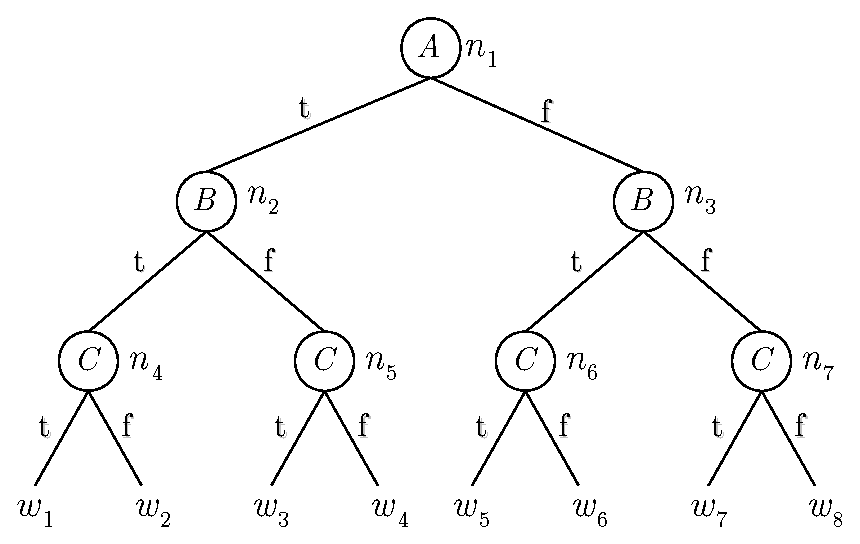
\includegraphics[width=\textwidth]{search_tree}
	\caption{A search tree for the CNF $\Delta =\{\{\neg A,B\},\{\neg B,C\}\}$.}
	\label{fig:searchtree}
\end{figure}

%\subsubsection{Depth-first-search algorithm}

\begin{algorithm}
\textsc{Depth-first-search}(CNF $\Delta$,depth $d$):\\
\uIf{$\Delta=\{\}$}{
	\bf{return \{\}}.
}
\uElseIf{$\{\}\in \Delta$}{
	\textbf{return} \textsc{unsatisfiable}
}
\uElseIf{\textsc{\textbf{L}}$=$\textsc{Depth-first-search}$(\Delta |P_{d+1},d+1)\neq$\textsc{unsatisfiable}}{
	\textbf{return} \textbf{L} $\cup$ $\{P_{d+1}\}$
}
\uElseIf{\textsc{\textbf{L}}$=$\textsc{Depth-first-search}$(\Delta |\neg P_{d+1},d+1)\neq$\textsc{unsatisfiable}}{
	\textbf{return} \textbf{L} $\cup$ $\{\neg P_{d+1}\}$
}
\Else{\textbf{return} \textsc{unsatisfiable}}
\caption{Depth-first-search algorithm. Variables are named $P_1,P_2,....$. Initial depth is 0.\label{dpll}}
\end{algorithm}    

%The Davis-Putnam-Logemann-Loveland (DPLL) \cite{dpll} algorithm is the base of all modern SAT solvers. Many refinements have been made to this algorithm over the last decade, which have been significant enough to change the behaviour of the algorithm, but it is still important to know it for understanding modern solvers. Figure ~\ref{fig:searchtree} shows a search tree with three variables. 

\begin{exmp}[Depth-first-search]$ $
\newline
Consider the CNF of Figure \ref{fig:searchtree} and the node labelled $n_5$. At this node, Algorithm ~\ref{dpll} will condition $\Delta$ on literals $A,\neg B$, leading to:
\[\Delta |A,\neg B=\{ \{\textbf{false},\textbf{false}\},\{\textbf{true},C\}\}=\{\{\}\}.\]
The algorithm will detect that there is a contradiction at this internal node, hence concluding that neither $w_3$ or $w_4$ are models of $\Delta$, without having to visit them explicitly. The algorithm can also detect success at internal nodes, implying that all assignments from that particular node are models of the CNF.
\end{exmp}

%\newline
%\newline
\noindent
\textbf{Unit resolution}
\newline
\newline
\noindent
One of the downsides of Algorithm \ref{dpll} is that we still have to search deeper into the search-tree than we really need to. The \textit{unit resolution} (also called \textit{unit propagation}) technique allows us to prune the search tree at each decision level. The unit resolution technique is very simple: Before we check tests for success or contradictions, we first collect all unit clauses. Then we assume that the variables which make these clauses unit are set to satisfy the unit clauses. Finally, we simplify the CNF and check for success or failure.

\begin{exmp}[Unit resolution]$ $
\newline
Consider the tree of Figure ~\ref{fig:terminationtree} and the CNF:
\[\Delta=\{\{\neg A,B\},\{\neg B,\neg C\},\{C,\neg D\}\}.\]
Consider also the node at Level 1, which results from setting variable A to \textbf{true}, and its corresponding CNF:
\[\Delta |A=\{\{B\},\{\neg B,\neg C\},\{C,\neg D\}\}.\]
Algorithm ~\ref{dpll} cannot declare early success or early failure, because the CNF is neither empty, nor contains the empty clause, reason why it keeps searching below Level 1 as shown in Figure \ref{fig:terminationtree}. However, by using unit resolution, we can declare success and end the search at Level 1. Because the clause $\{B\}$ has become unit, we can assume that variable $B$ is \textbf{true}. Now the clause $\{\neg B, \neg C\}$ is simplified to $\{\neg C\}$ (because $\neg B$ is \textbf{false} and cannot satisfy the clause) which is a unit clause. This will cause $C$ to be \textbf{false} and clause $\{C,\neg D\}$ to be simplified to $\{\neg D\}$. This clause is also unit now so $D$ must be assigned \textbf{false} and hence all clauses in this CNF have been satisfied through unit resolution. We can then declare that success without having to go any further in the search tree. Remember that the unit resolution process is very fast and does not require to make any decisions.
\end{exmp}

\begin{figure}[h!]
	\centering
		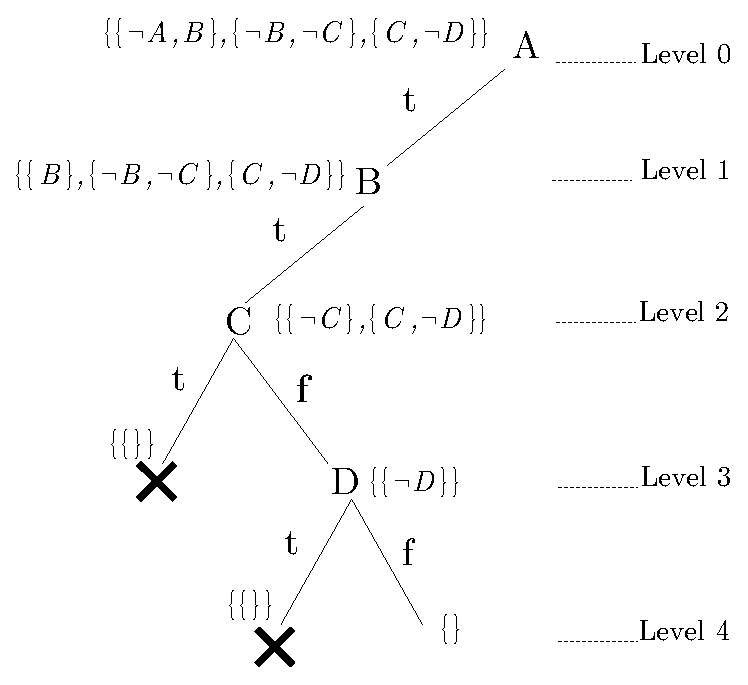
\includegraphics[width=0.7\textwidth]{termination_trees}
	\caption{A termination tree, where each node is labelled by the corresponding CNF. The last node visited during the search is labelled with \{\}. The black crosses indicate the detection of a contradiction at that node.}
	\label{fig:terminationtree}
\end{figure}

To incorporate the advantages of unit resolution into Algorithm \ref{dpll}, we will introduce a function \textsc{unit-resolution}, which applies to a CNF $\Delta$ and returns two results:
\begin{itemize}
	\item \textbf{I}: a set of literals that are either present as unit clauses in $\Delta$, or were derived from $\Delta$ by unit resolution.
	\item $\Gamma$: a new CNF which results from conditioning $\Delta$ on literals \textbf{I}.
\end{itemize}

\begin{exmp}[unit-resolution function]$ $
\newline
If the argument of \textsc{unit-resolution} was the CNF
\[\Delta=\{\{\neg A,\neg B\},\{B,C\},\{\neg C,D\},\{A\}\},\]
then $\textbf{I}=\{A,\neg B,C,D\}$ and $\Gamma=\{\}$. Moreover, if
\[\Delta=\{\{\neg A,\neg B\},\{B,C\},\{\neg C,D\},\{C\}\},\]
then $\textbf{I}=\{C,D\}$ and $\Gamma=\{\{\neg A,\neg B\}\}$.
\end{exmp}

%\newline
%\newline
\noindent
\textbf{DPLL algorithm}
\newline
\newline
\noindent
The DPLL algorithm (Algorithm \ref{dpllplus}) is a refinement of the depth-first-search algorithm. The first change made is that it adds unit resolution in line 1. Also, we no longer assume that variables are examined in the same order as we go down the search tree and we no longer assume that a variable is set to \textbf{true} and then to \textbf{false}. The choice of a literal $L$ on line 7 can have a dramatic impact on the running time of DPLL. This is where inference comes into play when solving a SAT instance with a DPLL based algorithm, heuristics and random factors are commonly used at this point. 

Note that DPLL algorithm will check, even if not implicitly, all leafs of the search tree until an assignment that satisfies the CNF is found, or until all leafs have been discarded and no assignment that satisfies the CNF is found. Furthermore, it will never visit the same node of the search tree more than once (it will not make the same decision sequence twice). Therefore, algorithm DPLL is complete.

\begin{algorithm}
$(\textbf{I},\Gamma)=\textsc{unit-resolution}(\Delta)$\\
\uIf{$\Gamma=\{\}$}{
	\bf{return \textbf{I}}.
}
\uElseIf{$\{\}\in \Gamma$}{
	\textbf{return} \textsc{unsatisfiable}
}
\Else{
	choose a literal $L$ in $\Gamma$\\
	\uIf{$\textbf{\textsc{L}}=\textsc{dpll}(\Gamma |L) \neq \textsc{unsatisfiable}$}{
		\textbf{return} \textbf{L} $\cup$ \textbf{I} $\cup$ $\{L\}$	
	}
	\uElseIf{$\textbf{\textsc{L}}=\textsc{dpll}(\Gamma |\neg L) \neq \textsc{unsatisfiable}$}{
		\textbf{return} \textbf{L} $\cup$ \textbf{I} $\cup$ $\{\neg L\}$	
	}
	\Else{
		\textbf{return} \textsc{unsatisfiable}
	}
}
\caption{DPLL(CNF $\Delta$): returns a set of literals or \textsc{unsatisfiable}\label{dpllplus}}
\end{algorithm}    

\subsubsection{Conflicts}

A \textit{conflict} occurs when a variable value assumption leads to an unsatisfiable CNF. In the DPLL algorithm this happens when we make a literal choice (in line 7 of Algorithm \ref{dpll}) and then the algorithm realizes that the new CNF that includes such assumption is unsatisfiable. In this case the algorithm will \textit{backtrack} the decision (undo the assignment) and try with another value. Because of the recursive nature of the DPLL algorithm, we should notice that the backtracking done is always the exact inverse order as the order in which we made the assignments. For example, if an assignment $\Delta | A,B,C,D$, made in that same particular order, leads to a contradiction, then the algorithm would backtrack the last decision made and undo the $D$ assignment. It will now try the $\neg D$ assignment, but if it also proves to lead to a contradictions, then it will also backtrack this decision. At this point it is implied that $\Delta | A,B,C$ is also a contradiction, but note that the DPLL algorithm did not detect the contradiction here (could only imply it after making the $D$ and $\neg D$ assignments). Now the algorithm will also backtrack the $C$ assignment and try $\neg C$. As we have seen in this brief example, the backtracking is always done in the same order that the assignments were done.

\subsubsection{Chronological backtracking}

As it was shown earlier, when we detect a conflict at level $l$ of the search tree, we have to rewind back to level $l-1$, undoing all assignments made in the process. Then we try another value at level $l-1$, if none remains  to be tried, we then go back further to level $l-2$, and so on. If we ever reach level $0$ and each value there leads to a contradiction, we will know that the CNF is inconsistent. This type of backtracking in the DPLL algorithm is called \textit{chronological backtracking}, because we move back in the same order we got there; one level at a time. 

\subsubsection{Non-Chronological backtracking}

The problem with chronological backtracking, which is the one used in the DPLL algorithm, is that contradictions that trigger the backtrack often have valuable information. Such information could lead us to learn new clauses and backtrack more levels than just one, thus saving time in the search. For example, let us say that we have a CNF $\Delta$ with variables $A,B,C,D$. Let us also say that, because of the clauses in $\Delta$, the CNF will always be inconsistent when $A$ is set to \textbf{true}. Unfortunately, the DPLL algorithm might not realise this beforehand, because it uses unit resolution which is not refutation complete. So the algorithm might only conclude that $A$ set to \textbf{true} will not satisfy $\Delta$ after assigning all possible values to $B,C,D$. If we could detect that $A$ is not part of any solution, we could avoid going any further in that branch of the search tree and learn that information as a new clause (in our example we would learn the clause $\{\neg A\}$ to enforce $A$ to be \textbf{false}). Learning such clauses is called \textit{conflict-driven clause learning} (CDCL) \cite{cdcl1,cdcl2}.

This new version of the DPLL algorithm is also complete. It is not so obvious that completeness is maintained, because now the algorithm, unlike the basic DPLL version, can make the same decisions more than once (visit a node in the search tree various times), since it does not maintain memory of the previous decisions made. However, it does so in a different context, because it has learned clauses since its previous visits to the same node. This guarantees that completeness in this new algorithm is maintained. A completeness proof of the DPPL algorithm with CDCL features can be found in \cite{DBLP,ig}. In the next section we will discuss in detail how such new clauses are found or how can we decide which level to backtrack after a contradiction is found.

\subsubsection{Clause learning}

When a conflict is detected, the conflict-analysis procedure is used. Such procedure consists of analyzing the conflict structure through \textit{implication graphs} and then learning a clause from it. Let's consider the following CNF:

\begin{equation}\label{row sum}
\Delta = \begin{matrix*}[l]
			1.\{A,B\}\\
		 	2.\{B,C\}\\
		 	3.\{\neg A,\neg X,Y\}\\
		 	4.\{\neg A,X,Z\}\\
		 	5.\{\neg A,\neg Y,Z\}\\
		 	6.\{\neg A,X,\neg Z\}\\
		 	7.\{\neg A,\neg Y,\neg Z\}
		 \end{matrix*}
\end{equation}

The implication graph on Figure \ref{fig:uip} shows a possible search path of a CDCL solver. The nodes of this graph are variable assignments made, with the notation $l/V=v$, where $l$ is a decision level, $V$ a variable and $v$ a truth value. Remember that a variable might be assigned a value in two cases: by a branching decision or by an implication as a result of the propagation process. The directed edges in the graph indicate which assignments implicated other assignments, so an edge from node $\alpha$ to node $\beta$ would mean that the variable assignment in node $\alpha$ implies the assignment shown in node $\beta$. Nodes that do not have any incident edge are decision assignments, because they weren't implied by other assignments. The numeric label on the arcs correspond to the number of the clause that was used for implying that assignment. 

\begin{figure}[h!]
	\centering
		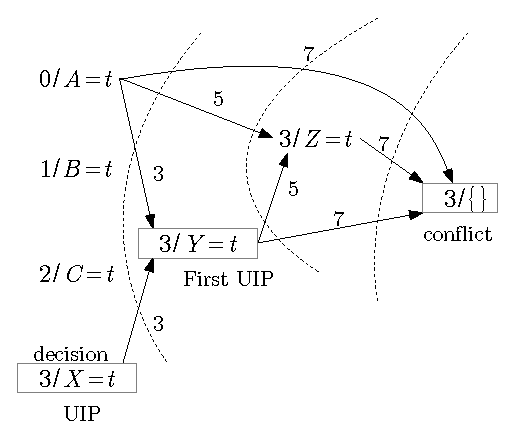
\includegraphics[width=0.7\textwidth]{uip}
	\caption{An implication graph of a conflict}
	\label{fig:uip}
\end{figure}

A \textit{cut} in an implication graph (dashed lines in Figure \ref{fig:uip}) is a set of edges that separate the decision assignments (root nodes) from the contradiction (the leaf node containing $\{\}$). A \textit{conflict set} is a set of variable assignments such that each has an outgoing edge belonging to the same cut, in other words, a conflict set contains enough variable assignments to cause the conflict \cite{grasp,cdcl1,ig}. Figure \ref{fig:uip} shows three possible cuts for that implication graph, they lead to the conflict sets $\{A=\textbf{true},X=\textbf{true}\}$, $\{A=\textbf{true},Y=\textbf{true}\}$ and $\{A=\textbf{true},Y=\textbf{true},Z=\textbf{true}\}$.

Since there are many possible cuts, and thus conflict sets, we are only interested in choosing the most useful ones. An \textit{asserting clause} \cite{cdcl1} is a clause derived from a conflict set (containing the negation of the assignments in the conflict set) which contains exactly one variable assigned at the level of the conflict. From the previous conflict sets, $\{\neg A,\neg X\}$ and $\{\neg A,\neg Y\}$ are asserting clauses, because only $X$ and $Y$ were decided at the conflict level. 

A refinement to the definition of an asserting clause is the notion of a \textit{unique implication point} (\textit{UIP}) \cite{grasp,cdcl1}. A UIP of a decision level is a variable which was set at that level and that lies in every path from the decision variable at that level to the conflict. For example, the assignments $3/Y=\textbf{true}$ and $3/X=\textbf{true}$ are both UIPs of level 3, and $0/A=\textbf{true}$ is a UIP of level 0. UIPs of a decision level can also be given an order, the first UIP is the one closest to the contradiction. In Figure \ref{fig:uip} the first UIP of level 3 is $3/Y=\textbf{true}$. The \textit{1UIP scheme}, used in modern solvers, learns asserting conflict-driven clauses which have the first UIP of the decision level of the conflict. 

\subsection{Modern CDCL solvers}

Most modern solvers today are CDCL SAT solvers. Given a CNF $\varphi$, a partial assignment of variables $\nu$, Algorithm \ref{cdcl} outlines the general structure of a CDCL SAT solver, where $x$ is a variable, $v$ a truth value and $\beta$ a decision level. We will shortly explain the main functions of this algorithm.

\begin{algorithm}
\KwIn{A CNF $\varphi$ and a variable assignment $\nu$}
\If{\textsc{(UnitPropagation($\varphi$,$\nu$)}=={\bf CONFLICT}\textsc{)}}{
	\bf{return UNSAT}.
}
$dl \leftarrow 0$\\
\While{\textsc{(}{\bf not} \textsc{AllVariablesAssigned($\varphi$,$\nu$))}}{
	\textsc{($x$,$v$)=PickBranchingVariable($\varphi$,$\nu$)}\\
	$dl \leftarrow dl+1$\\
	$\nu \leftarrow \nu$ $\cup$ \{($x$,$v$)\}\\
	\If{\textsc{(UnitPropagation($\varphi$,$\nu$)}=={\bf CONFLICT}\textsc{)}}{
		\textsc{$\beta$=ConflictAnalysis($\varphi$,$\nu$)}\\
		\uIf{\textsc{($\beta < 0$)}}{
			\Return{{\bf UNSAT}}
		}
		\Else{
			\textsc{Backtrack($\varphi$,$\nu$,$\beta$)}\\
			$dl \leftarrow \beta$
		}
	}
}
\Return{\textsc{\textbf{SAT}}}
\caption{Typical CDCL algorithm\label{cdcl}}
\end{algorithm}

\begin{itemize}
	\item \textsc{UnitPropagation} consists of iteratively deducing the truth value of variables. The values are deduced by logical reasoning on $\varphi$ and $\nu$. We already discussed this function in the previous sections.
	\item \textsc{PickBranchingVariable} consists of selecting a variable to assign, and the respective value. Heavily relies in heuristics/random factors to pick variables.
	\item \textsc{ConflictAnalysis} consists of analyzing the most recent contradiction and learning a new clause from it. It returns the decision level to backtrack to (non-chronological backtracking).
	\item \textsc{Backtrack} undoes variable assignments and backtracks to a previous decision level as computed by \textsc{ConflictAnalysis}.
	\item \textsc{AllVariablesAssigned} tests whether all variables have been assigned a truth value.
\end{itemize}


\subsubsection{The two watched literals lazy data structure}

Data structures play a fundamental role in the performance of CDCL SAT solvers. Many improvements have been achieved over the last years, but one of the most noticeable ones is use of the so called \textit{lazy data structures} (lazy because they are not accurate) to implement propagation. There are different types of lazy data structures used in modern SAT solvers, they mainly try to address cache performance problems when the solver is performing unit resolution. The two main approaches to implement lazy data structures are the \textit{head/tail lists} used in Sato \cite{sato} and the \textit{two watched literals} used in Chaff \cite{chaff}. We will explain the later in detail, as it is widely implemented in most modern CDCL SAT solvers.

\begin{figure}[h!]
	\centering
		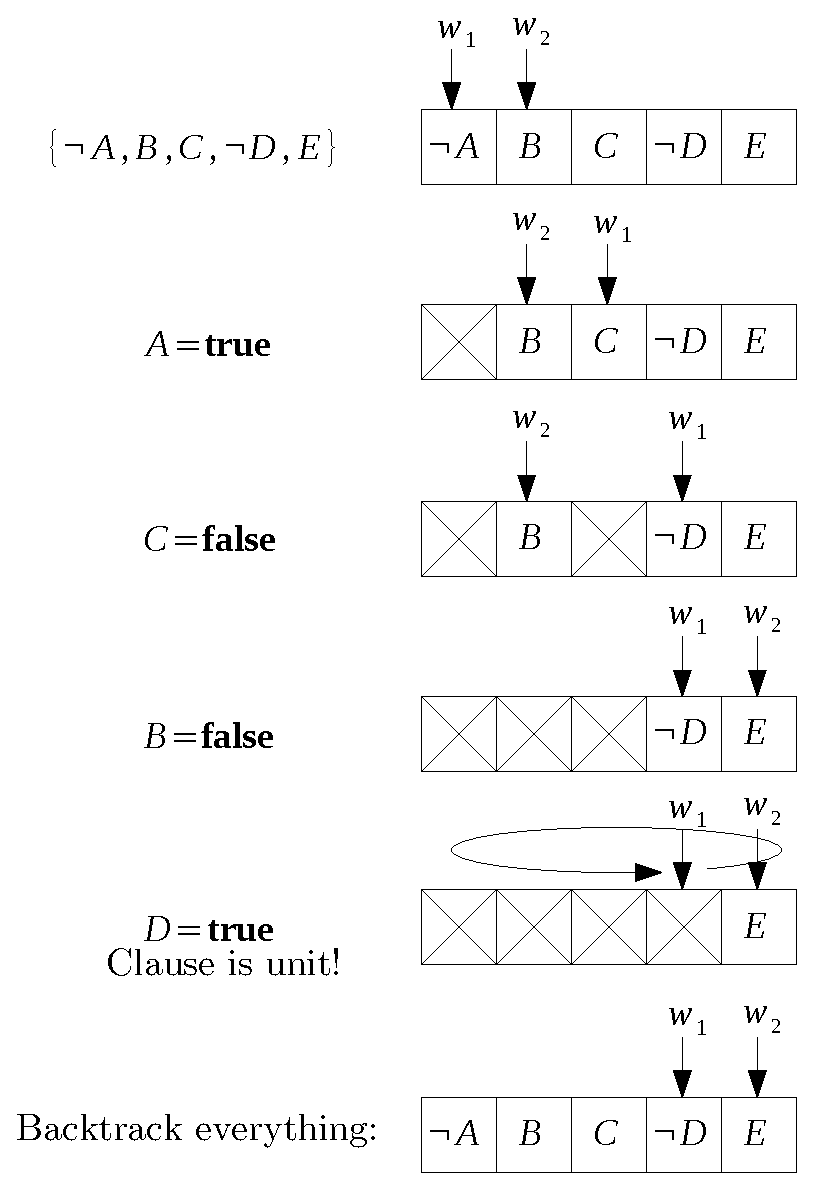
\includegraphics[width=0.5\textwidth]{watchedliterals}
	\caption{Operation of the two watched literal data structure.}
	\label{fig:watched literals}
\end{figure}

Unit propagation is a key function to the speed of a SAT solver. We need fast ways of identifying which clauses become unit when assigning variables. For example, if we have the clause
\[\{\neg A,B,C,\neg D,E\}\]
and the variable assignment
\[A=\textbf{true}, B=\textbf{false}, C=\textbf{false}, E=\textbf{false},\]
we would need to identify somehow that this clause is unit on variable $D$. The two watched literal data structure addresses this problem and makes backtracking very efficient. Instead of trying to keep precise information on the complete state of the clause, the two watched literal strategy only keeps track of two literals in each clause. Such two literals are the watched literals of a clause. Let's take as an example the previous clause, as shown on Figure \ref{fig:watched literals}. This time we will assume that no variable assignments have been done yet and that the two watched literals are $\neg A$ and $B$. Suppose that on the next decision level variable $A$ is assigned as \textbf{true}. We would check the watched literals and realize that this clause might be unit, because now there is only one watched literal which is unassigned and the other doesn't satisfy the clause. Remember that we are only aware of the watched literals and not the rest of them. To check if the clause is really unit, we will attempt to change the first watched literal to an unassigned variable in the clause. We could search to the right and find that literal $B$ is already being watched (the two watched literals must be different), so we keep searching to the right and find that literal $C$ is unassigned, concluding that the clause is not yet unit. Now our two watched literals for this clause are $B$ and $C$. Let's suppose now that propagation gives the value \textbf{false} to variable $C$, then we would again wonder if the clause is unit or not. Searching to the right for another unassigned literal to watch will find literal $\neg D$, so now our two watched literals will be $B$ and $\neg D$. If the next assigned variable is $B=\textbf{false}$, then the algorithm would have to search the clause and find that literal $E$ is available. Finally, if variable $D$ is assigned to \textbf{true}, then we would search the clause for an available literal, but won't find any (after checking all literals). Only now we can declare that this clause is unit, because there is only one unassigned watched literal and the other can't find any unassigned position. Propagation would assign \textbf{true} to variable $E$, because it's the only way to satisfy that clause. If a conflict is found, while propagating across the different variables, we have to undo all variable assignments after the backtracking point, but the key advantage of the two watched literal structure is that no backtracking has to be done to any watched literal reference of any clause. The clear drawback to this advantage is that, as we saw in the previous example, we have to check all literals in the clause before declaring it unit, since we only keep track of two literals at a time.  

\subsubsection{Binary implication lists}

\begin{figure}[h!]
	\centering
		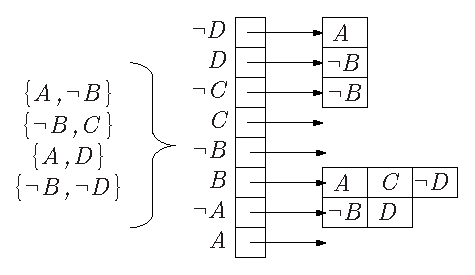
\includegraphics[scale=1]{binary_lists}
	\caption{A group of binary clauses and their corresponding binary list.}
	\label{fig:binary list}
\end{figure}

To speed up the propagation of SAT solvers, \textit{binary clauses}, clauses with two literals, are sometimes stored in special data structures called \textit{binary implication lists}. Binary clauses are frequently used in propagation because they can imply other variable values in just one step. There is also no point on distinguishing two watched literals in these clauses for the simple reason that there are only two literals in them, so knowing when a binary clause is unit becomes trivial. Figure \ref{fig:binary list} represents a set of binary clauses stored in a binary implication list. We have a literal index vector to identify each literal (a variable and its negation), each position of this vector points to a list of literals which are implied by the literal corresponding to the origin of the pointer. Hence, if the $\neg A$ position in the index vector points to $\neg B$ and $D$, this means that if $A$ were to be \textbf{false}, it would imply that $B$ must be \textbf{false} and $D$ \textbf{true}.

\subsubsection{Search restarts}

SAT solvers may exhibit high runtime variability on some problems. This means that some decision heuristics and random factors make the solver take a really long time in solving a problem, but others can help solve the same problem in a very short runtime. This phenomena exhibited by SAT solvers and these kind of problems is known as a \textit{heavy tailed distribution}. A heavy tailed distribution has infinite variance and infinite mean, so a SAT solver might get trapped on a very long run with a problem, while a different instance of the solver with other parameters could solve it fast. To address this problem modern SAT solvers have included search restarts in their solving algorithms. To avoid keeping the solver trapped in a very long search path, search restarts are issued over time and the solver starts the search all over again. In practice this strategy has shown dramatic improvements on problems which exhibit the heavy tailed behaviour \cite{heavytail}. It is also important to mention that learnt clauses can be kept between each restart, technique that can ensure the completeness of the algorithm under such search restarts (only one learnt clause in each iteration suffices to guarantee completeness\cite{LMS07}). 

\subsubsection{Variable decision heuristics}

There are several heuristics that can be employed when choosing a decision variable, even making this decision completely random, but the most popular one was introduced by the solver \texttt{Chaff} and it's called Variable State Independent Decaying Sum (VSIDS). This heuristic consists of the following:
\begin{itemize}
	\item Each literal has a counter, initialized to 0.
	\item The counter of a literal is only incremented in 1 when a new clause that contains that literal is learnt.
	\item When choosing a decision literal, the unassigned literal with the highest counter is chosen.
	\item Ties are broken by random.
	\item All counters are periodically divided by a constant.
\end{itemize}
\texttt{MiniSAT} \cite{minisat} later made some refinements to this heuristic and instead of keeping counters for each literal, it keeps it for each variable. It also uses a dynamic increment factor (not just by 1) and does not use a periodic decay constant, but just scales all values down when one of them has become too large. This refinement of VSIDS is known as Exponential VSIDS (EVSIDS). 

\subsubsection{Clause cleanup}

Adding clauses with no restrictions can be impractical in some cases. We could eventually exhaust all the available memory by learning too many clauses and it is also known that large clauses are not really useful in the search process \cite{grasp}. Large clauses also add some considerable overhead to the search process and it is sometimes better to get rid of them than to keep them. Because of this, there are mainly 3 techniques employed to keep the clause database manageable:

\begin{enumerate}
	\item Only keep clauses with $n$ or less literals \cite{dec90}.
	\item Clauses are kept only if they imply variable assignments or are unit clauses. They are discarded if the number of unassigned literals is greater than a number $m$ \cite{bs97}.
	\item Clauses with a number of literals greater than a threshold $k$ are discarded as soon as the number of unassigned literals is greater than one \cite{grasp}.
\end{enumerate}

Lately, some solvers have started using more advanced heuristics as clause deletion policies, such as keeping information about the activity of a clause in conflicts. One of the best performing heuristics is employed in the SAT solver \texttt{gluclose} \cite{gluclose}, which implements a particular metric of clause activity for its deletion heuristics.

\subsection{Parallel SAT solvers}

As mentioned before, some parallel SAT solvers have performed at the top of the last SAT competitions, but even though they all fall into the parallel solvers category, their parallel strategies and implementations vastly differ from each other. We mainly classify parallel SAT solvers into two categories: Portfolio approach solvers and divide-and-conquer ones.

The main idea behind portfolio approach solvers is the fact that different kinds of sequential solvers will perform differently for different kinds of SAT problems. The portfolio approach is a very straight forward strategy: They run a group of sequential solvers in parallel, each with different heuristic values and/or different search strategies. The time they take to solve the problem will be the time of the fastest solver in the group of solvers running in parallel. Although all portfolio approach solvers share this same principle, they also have quite different kinds of implementations. We identify in this group the solvers that do not share information, the ones that share clauses only logically, and the ones that share clauses physically and logically.

Solvers that do not share information have the most simple design. They run completely independent solvers in parallel and wait for one of them to give an answer. Despite their simplicity, the solver ppfolio \cite{ppfolio}, a pure portfolio approach solver, was the winner of the crafted and random categories of the 2011 SAT competition of parallel solvers, and second place in the application category. 

On the other hand, we have more elaborated portfolio approach solvers, which can also share clauses logically between their different solvers. One of the characteristics of CDCL solvers is the fact that they can learn new lemmas as they solve a SAT problem. These new lemmas will provide additional information during the solution search, so that the solver doesn't fall into previous fruitless search paths. The idea is that different solvers running in parallel can share their learned lemmas so that they all benefit from what other solvers have learned and improve their own search. An example of these kind of solvers is \texttt{ManySAT} \cite{manysat}, which won the 2009 SAT competition in the parallel solver application category. \texttt{ManySAT} has its own sequential state-of-the-art SAT solver and runs different instances of it in parallel, using different VSIDS \cite{vsids} heuristics (branching heuristics) and restart policies for each of it. The difference with pure portfolio approach solvers, is that \texttt{ManySAT} also shares learned lemmas between solving threads. It is called logical sharing of clauses, because the lemmas are passed as messages between threads and they never share the same physical information in memory. The advantage of logical sharing is that it is easier to implement message passing between threads, than having threads reading and modifying the same memory locations, which often requires locks that could hinder the overall solver performance. One of the best parallel performing solvers, \texttt{Plingeling} \cite{plingeling}, also shares clauses logically. It is a very weak sharing though, since it only shares unit lemmas and it does so through message passing, using a master thread to coordinate messages between worker threads. 

Portfolio approach solvers that share clauses physically have the same strategy as mentioned before, but they share clauses by allowing threads to access the same memory locations, instead of message passing. One solver in this category is \texttt{SArTagnan} \cite{sartagnan}, which shares clauses logically and physically. 

Divide-and-conquer solvers do not try to run different solvers in parallel, they run one solving instance, but try to parallelize the search and divide it between the different threads. A common strategy to divide the search space is to use \textit{guiding paths}. A guiding path is a partial assignment of variables which restricts the search space of the SAT problem. A solver that divides its search space with guiding paths will assign threads to solve the CNF with the given partial assignment from the guiding path the thread was assigned with. Once a thread finishes searching a guiding path with no success, it can request another to keep searching. \texttt{MiraXT} \cite{miraxt} is a divide-and-conquer SAT solver which uses guiding paths. Moreover, different threads solving different guiding paths also share a common clause database, in which they store their learned lemmas. This is another example of physical clause sharing. 

\subsubsection{MiraXT}

\begin{figure}[h!]
	\centering
		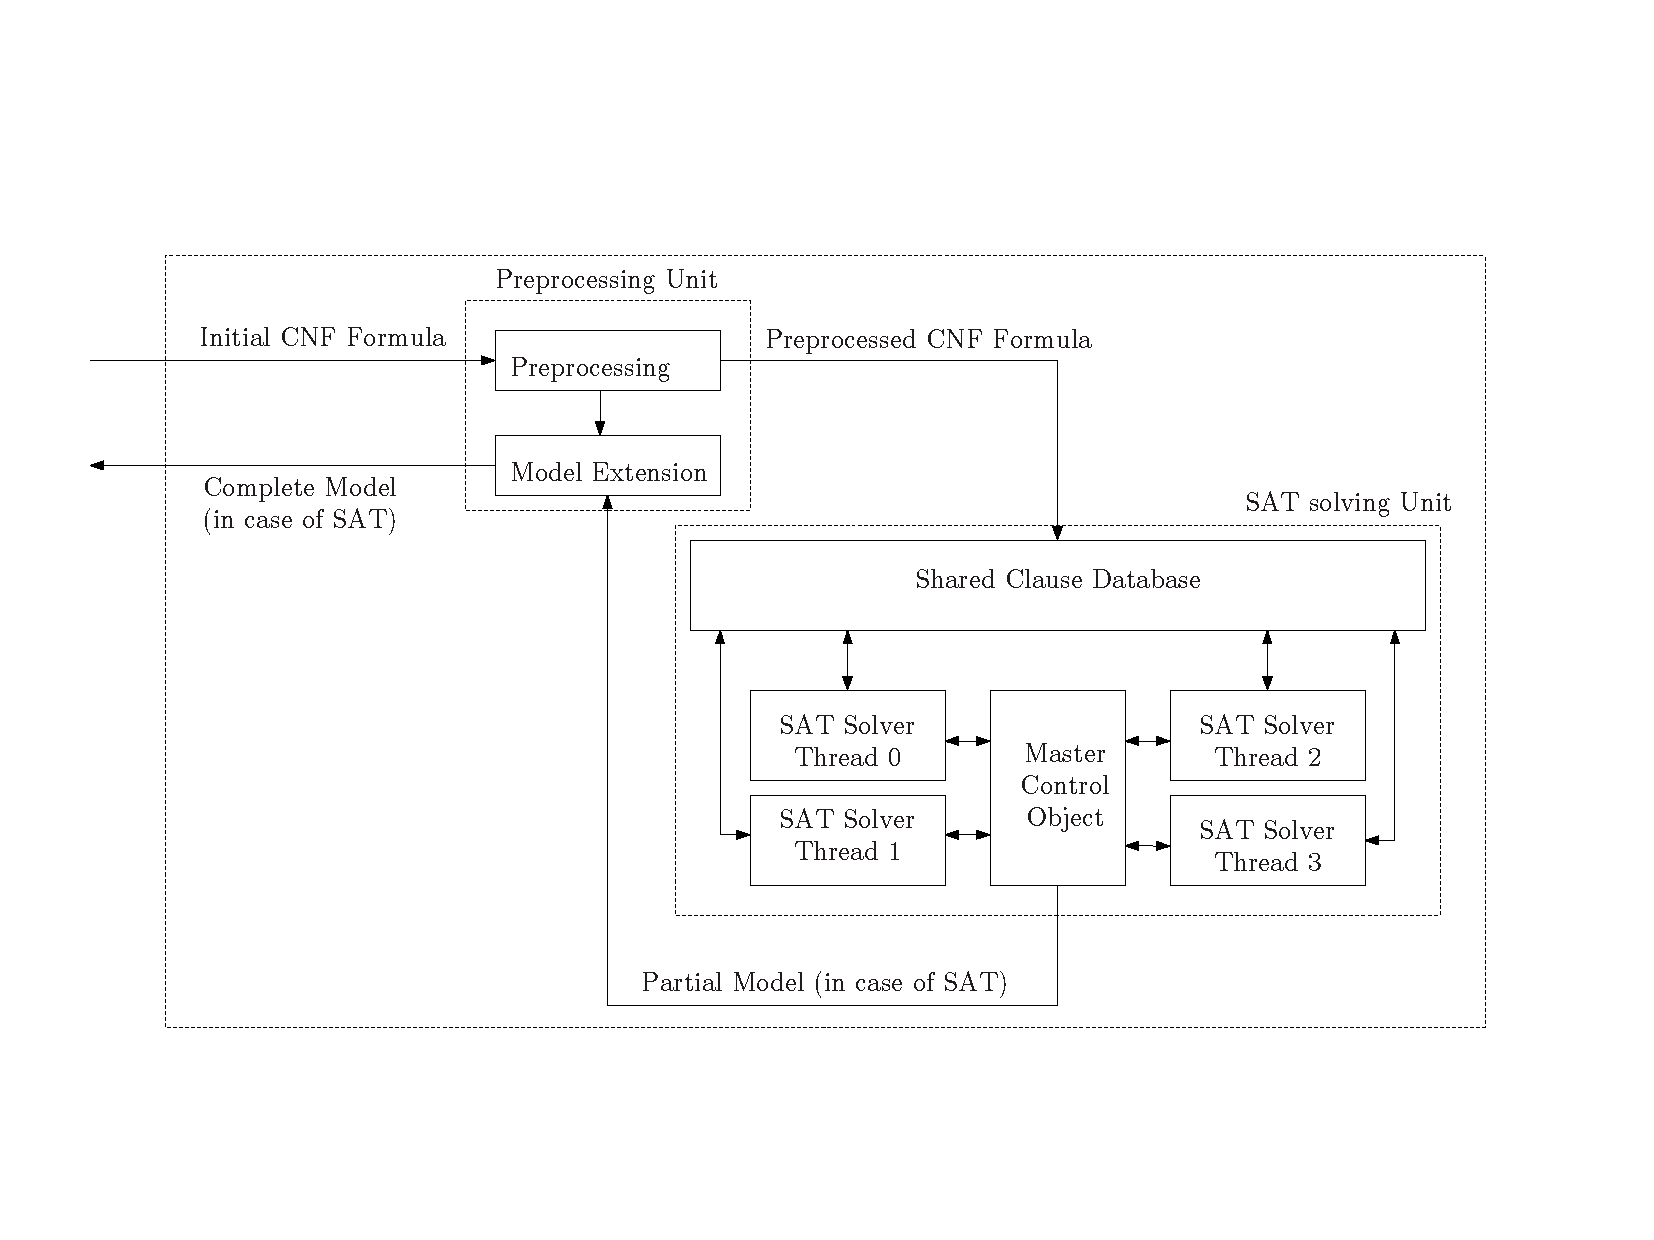
\includegraphics[width=\textwidth]{miraxtdesign}
	\caption{Overview of \texttt{MiraXT} design.}
	\label{fig:miraxt overview}
\end{figure}

Figure \ref{fig:miraxt overview} shows the general structure of the \texttt{MiraXT} solver, in which our solver AzuDICI bases its organization. We are not interested in the \textit{Preprocessing Unit} as it will not be implemented in our solver. The \textit{SAT Solving Unit} is of interest for our work though. The key structure in this design is the \textit{Shared Clause Database}, which is a database of clauses shared among all SAT solving threads. We will also be using this design in our solver, so all threads will be using a common pool of clauses called Shared Clause Database. The main difference with our design is that we will not have a \textit{Master Control Object} (MCO) structure, which in \texttt{MiraXT} is responsible for the coordination of different threads. The reason for this is that, as we mentioned earlier, MiraXT is a divide-and-conquer solver, so different threads will contribute to one solution and hence will need to be coordinated between each other in this task. On the other hand, our solver will be a portfolio approach one, so different threads will not need to interact with each other directly and no coordination between them is needed.

\begin{figure}[h!]
	\centering
		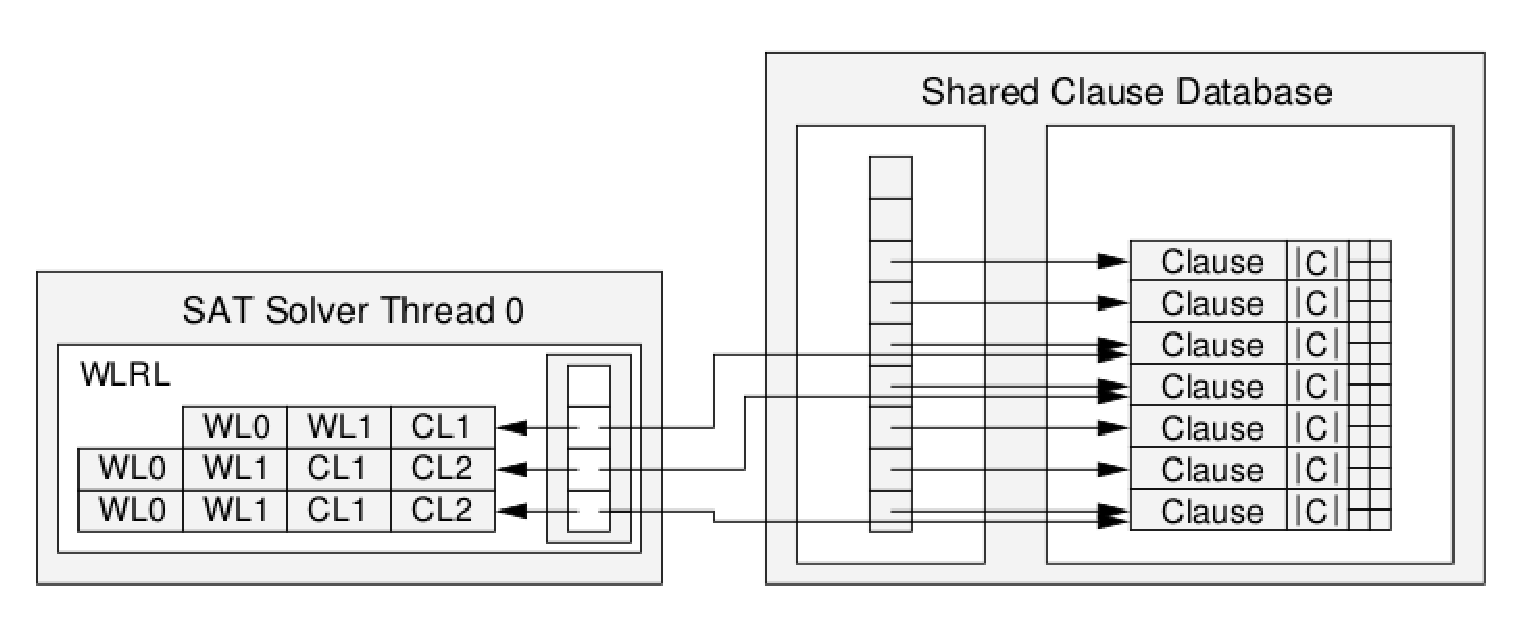
\includegraphics[scale=0.6]{miraxtdatabase}
	\caption{\texttt{MiraXT} shared clause database.}
	\label{fig:miraxt database}
\end{figure}

Figure \ref{fig:miraxt database} shows a representation of the shared clause database. Each thread keeps track of the two-watched-literals for the clauses it uses, and it also keeps two \textit{Cache Literals}, which serve to replace any of the watched literals that need to be updated, so that we do not need to load them from the shared clause database. If none of the Cache Literals would serve, then they would need to be updated too from the original clauses in the Shared Clause Database. Each clause in each thread has a pointer to the original clause in the Shared Clause Database, so that it knows where to update the Cache Literals from. The Shared Clause Database is read only, so locks are only used when a new clause is inserted, authors mention that lock contention only account for less than $1\%$ of total solving time.

To solve a problem \texttt{MiraXT} will start an initial thread solving the entire problem and depending on whether or not there are idle threads waiting, it will divide the problem into subproblems, with the guiding path technique, and share it with any idle thread. All communication and coordination between threads is done through the MCO with message passing, as shown in Figure \ref{fig:miraxt overview}. 

\section{Cache}

\begin{figure}[h!]
	\centering
		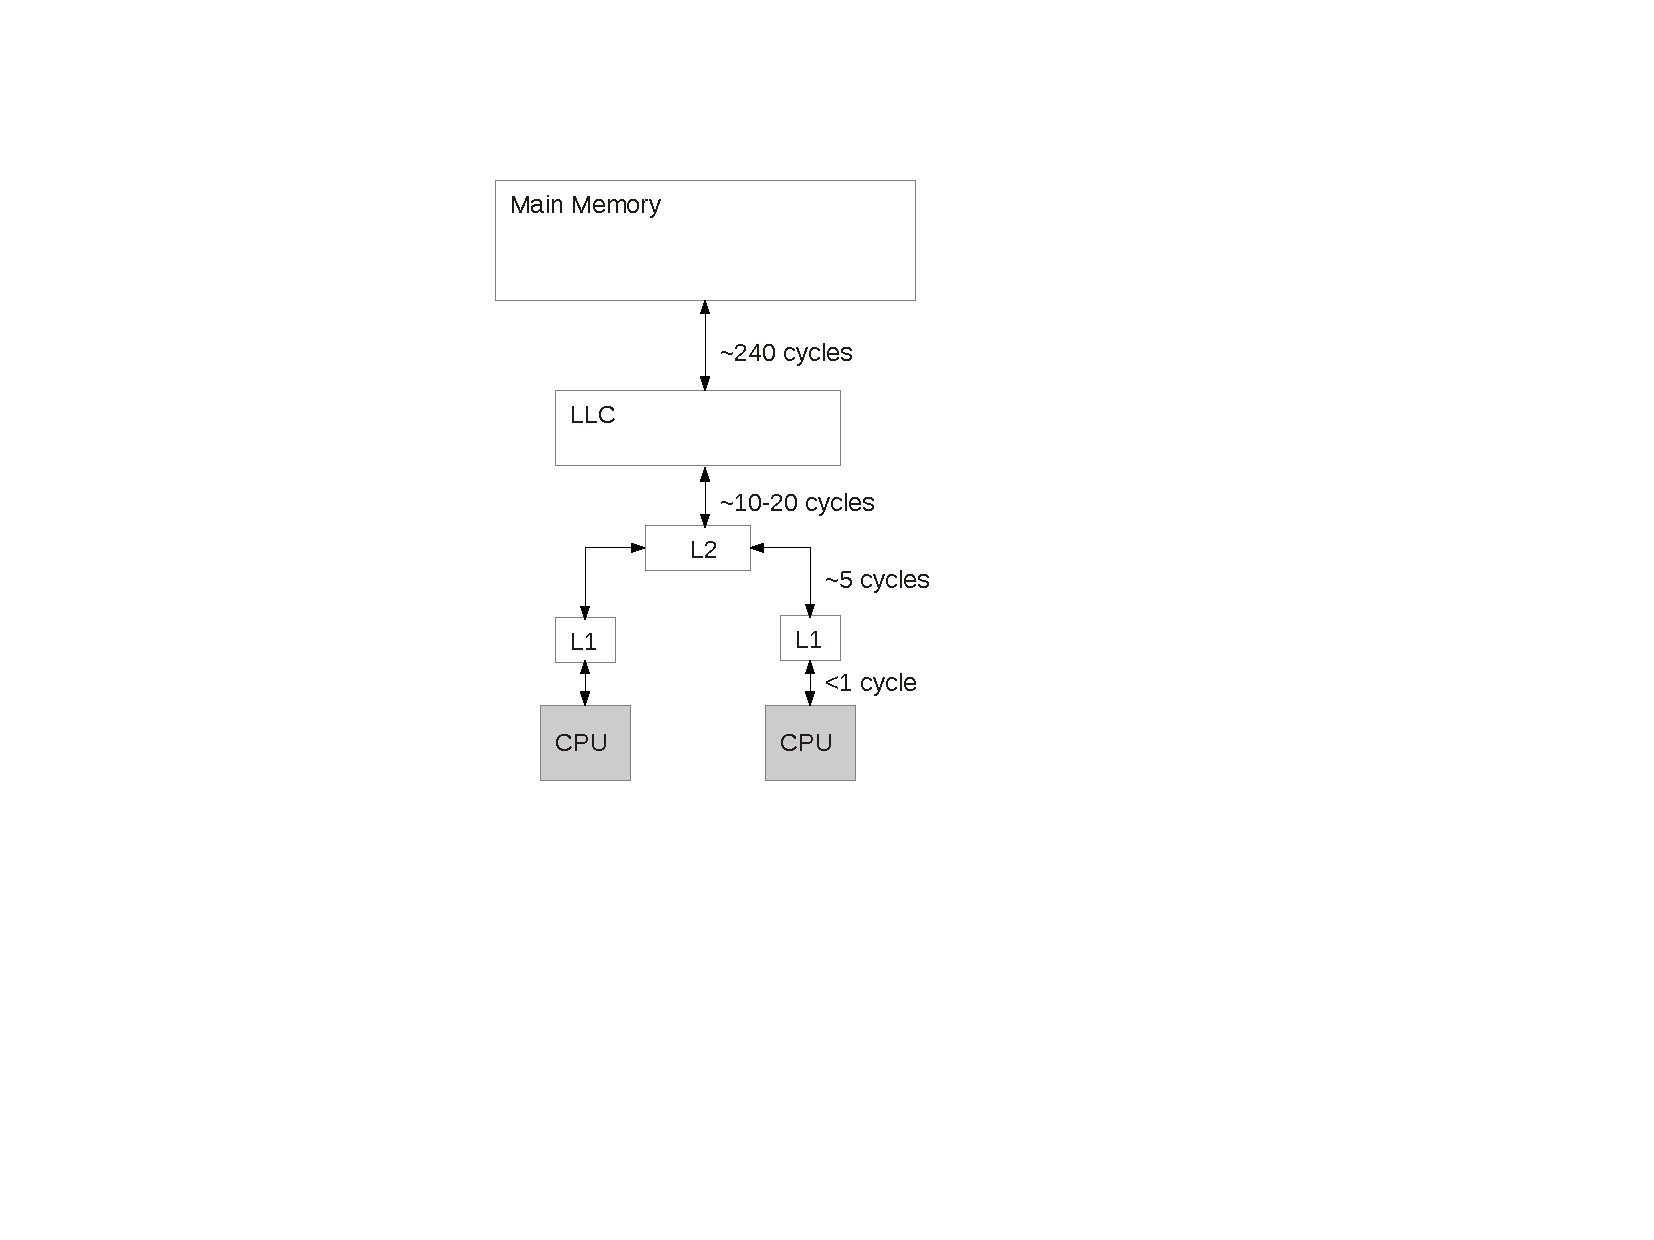
\includegraphics[scale=1]{cache}
	\caption{Typical memory hierarchy of modern computers.}
	\label{fig:cache}
\end{figure}

Computers today usually have three levels of memory cache and a main memory. The processor can have multiple cores in it and cores can run multiple threads in them. The difference between a core and a thread is that cores have separate copies of almost all the hardware resources. The cores can run independently unless they are using the same resource (for example the connection to the outside) at the same time. Threads, on the other hand, share almost all of the processor resources. When a thread, which is running on a core, needs to fetch data, it first tries to look for it in the first level cache (the L1 cache\footnote{There is L1 data cache and also L1 instruction cache, we will be referring to L1 data cache}), if the data is not there, then it tries to find it in the level 2 cache (L2 cache). If the data is still not there, it then tries to fetch it from the level 3 cache (L3 cache) and if that fails too, it goes up to main memory to get the data. If it still isn't in main memory, then it has to retrieve it from the hard disk. We should notice that this hierarchy involves increasing fetch times as we go up. Getting data from the L1 cache is much faster than getting it from L2, and getting data from L2 is much faster than getting it from main memory. The problem with lower level memory is that, because of the technology and costs involved, they are much smaller. So the big picture is that at lower levels we have faster and smaller memories, and at higher levels we have massive and slower memory storages. Figure \ref{fig:cache} is a schematic of today's computer memory hierarchy. To get an idea of the times involved in accessing data from different memory storages, we present the following table of costs associated with hits and misses, for an Intel Pentium M:
\begin{center}
\begin{tabular}{ c | c }
  To where & Cycles \\ \hline
  Register & $\leq 1$ \\
  L1 & ~3 \\ 
  LL & ~14 \\
  Main Memory & ~240 \\
\end{tabular}
\end{center}
 
\subsection{Cache and algorithms} 
 
Another important topic to discuss is how these memory caches operate. When data is requested and it is not found in any of the three caches, it has to be loaded from main memory. Data is not transferred individually, instead, a fixed amount of bytes containing the data (or part of it if it's large) is fetched. This fixed amount of bytes is called a \textit{word} or \textit{cache line}. Intel uses an \textit{inclusive} memory cache protocol, which loads a requested word from main memory into all cache levels. 
Because transferring data from main memory is so costly (compared to any cache level), we would like to transfer the highest amount of useful data from main memory to cache every time. Since the access times to any cache are so little compared to main memory, we will assume the bottleneck of data-fetching performance is main memory. 

\begin{algorithm}
\KwIn{A matrix $M$ of size $m \times n$, which elements are integers}
$sum \leftarrow 0$ \\
\For{$i\leftarrow 0$ \KwTo $m$}{
	\For{$j\leftarrow 0$ \KwTo $n$}{
		$sum=sum+M[i][j]$
	}
}
\Return{sum}
\caption{Row sum of elements\label{matrix row}}
\end{algorithm}

\begin{algorithm}
\KwIn{A matrix $M$ of size $m \times n$, which elements are integers}
$sum \leftarrow 0$ \\
\For{$i\leftarrow 0$ \KwTo $n$}{
	\For{$j\leftarrow 0$ \KwTo $m$}{
		$sum=sum+M[j][i]$
	}
}
\Return{sum}
\caption{Column sum of elements\label{matrix column}}
\end{algorithm}

Data-fetching performance is not only an issue that concerns hardware designers, but also programmers. Depending on how the program is written, the same task (input-output wise) might take much longer if one is not aware about how memory behaves. Since we want the highest amount of useful data in each word transferred, the data structures in which the programmer decides to store data will have a dramatic impact in cache performance. Consider, for example, the following problem: Write a program that sums all elements in a matrix size $m \times n$ of integers. Algorithm \ref{matrix row} and \ref{matrix column} both solve the problem, and apparently with the same level of efficiency, from an algorithmic point of view at least. However, the actual results of both algorithms in practice have a vast difference in total solving time. The following table shows the results for both algorithms implemented in C, for a matrix of size $31000 \times 31000$:
\begin{center}
\begin{tabular}{ c | c }
  Algorithm & Elapsed time (seconds) \\ \hline
  Row sum & 2.8 \\
  Column sum & 28.3 \\ 
\end{tabular}
\end{center}

Figure \ref{fig:matrixmemory} shows a representation of how matrix $M$ could be stored in main memory. As you can see, elements that are in the same row are stored in contiguous memory locations, while elements that are in different columns might be far away from each other. As we mentioned earlier, when an instruction requests data, it will bring a whole word that contains all or some of the data, from main memory to the cache. If we assume that the word size for our example is five integers, then when we fetch element $a$ of the matrix, we will also be fetching the whole row together. If Algorithm \ref{matrix row} is being executed, then after using element $a$, we will need element $b$, but since we already loaded the whole row into cache, there is no need to fetch $b$ from main memory! Same would happen with values $b$, $c$, $d$ and $e$. If, on the other hand, we were executing Algorithm \ref{matrix column}, after using element $a$ we would need to fetch element $f$, but element $f$ was not loaded in cache, so we will need to fetch another word from main memory that contains the $f$ element. Let's suppose now that we only have one level cache and that it can only hold one word at a time (remember cache is much smaller than main memory). Since the cache is full with the word that contains element $a$, we will need to \textit{evict} this word. Evicting a word means pushing it back to main memory and marking the cache line as usable. Once the word containing element $a$ is evicted from cache, we can then proceed to fetch the other cache line containing element $f$. After we have used element $f$, we will then need element $b$ (because we are performing a column sum) and hence produce another eviction and access to main memory. In this simple example, the final count of main memory accesses for Algorithm \ref{matrix row} is two, while for Algorithm \ref{matrix column} is ten. 

\begin{figure}[h!]
	\centering
		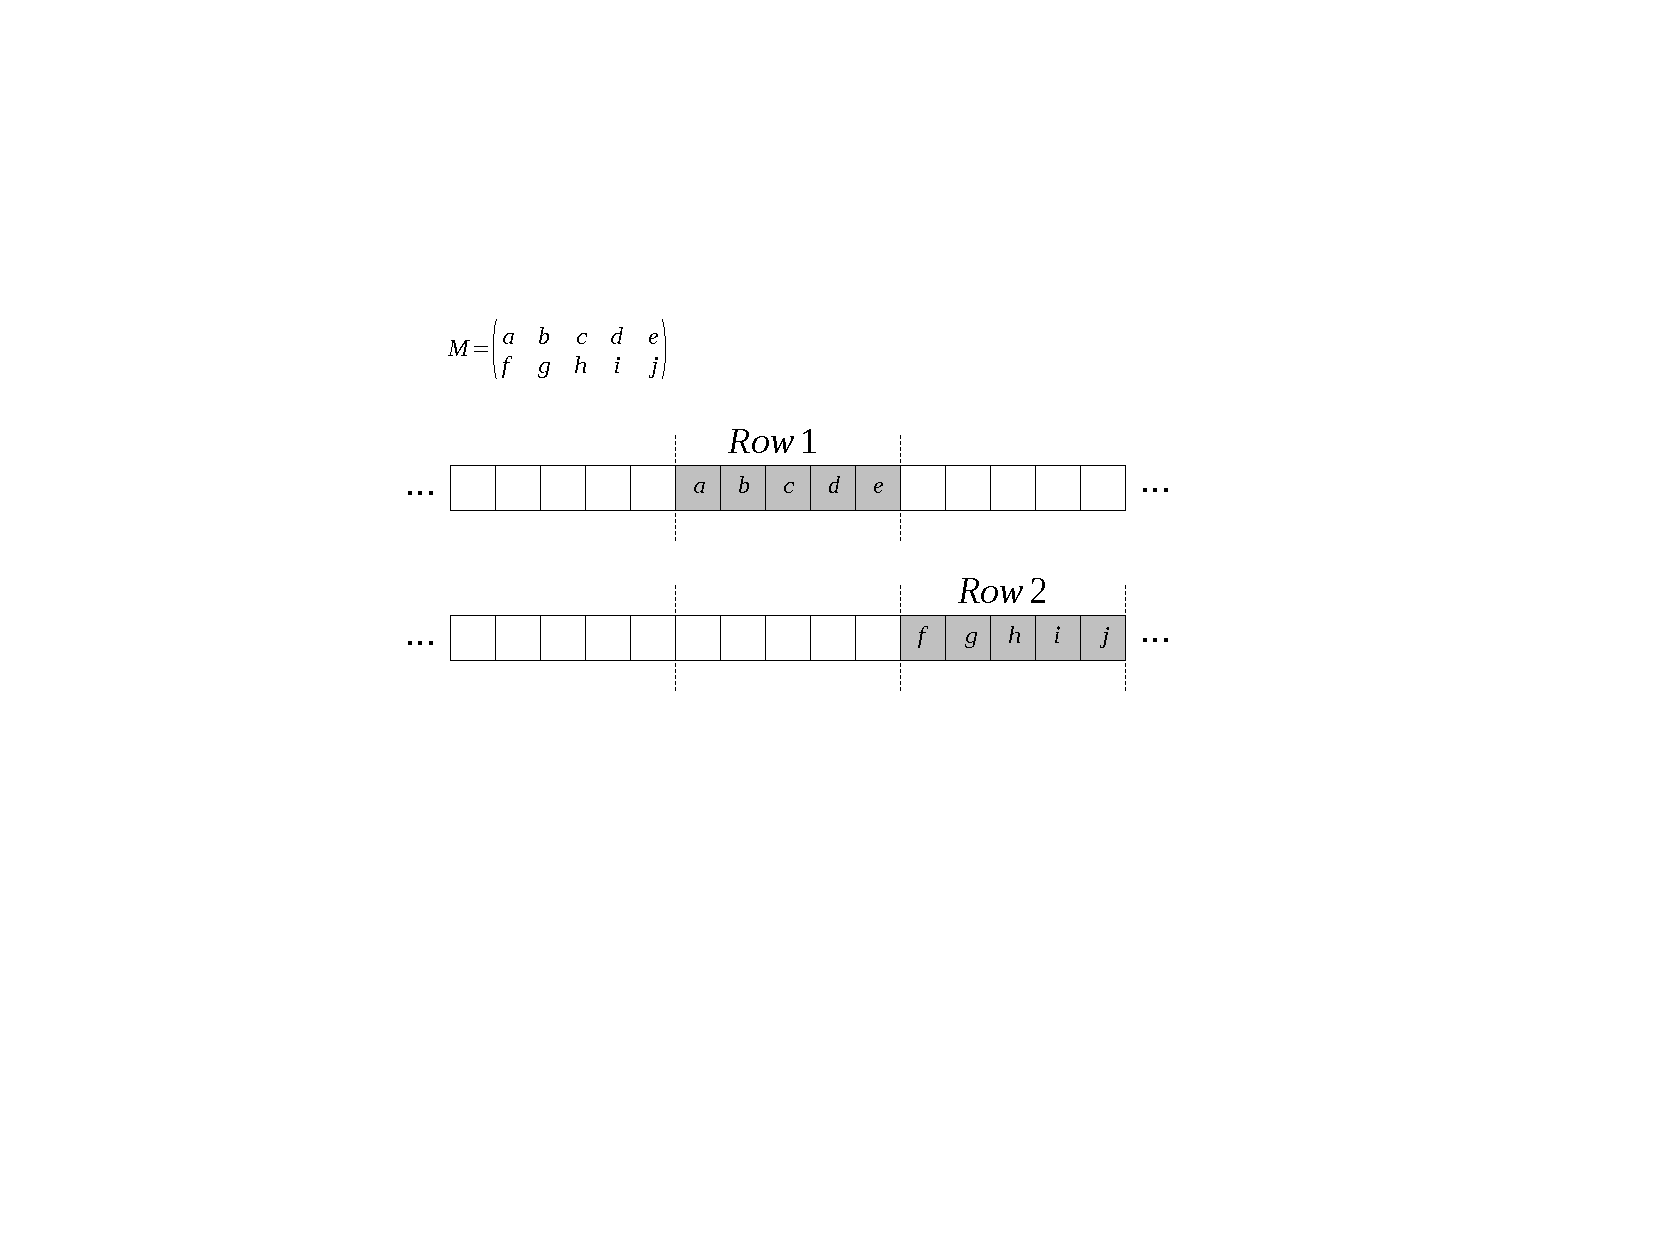
\includegraphics[width=0.7\textwidth]{matrixmemory}
	\caption{A representation of matrix $M$ in main memory.}
	\label{fig:matrixmemory}
\end{figure}

If we generalize our previous example to any matrix size, any word size and any cache size, we have the following formula to calculate the maximum amount of main memory accesses in Algorithm \ref{matrix row}:

\begin{equation}\label{row sum}
t=\left (\frac{n}{w} + 1 \right) \cdot m
\end{equation}

Where $t$ is the number of accesses to main memory, $w$ the word size, $n$ the number of rows of the matrix and $m$ the number of columns. Equation \eqref{row sum} does not take into account the cache size since it will always need to transfer each word containing the rows once. In the big-oh notation, we would have that:

\[ O(t)=\frac{n \cdot m}{w} \]

For Algorithm \ref{matrix column}, the formula to calculate the amount of transfers could be:

\begin{equation}\label{column sum}
t=(n \cdot m) - \left(\left(\frac{c}{w}-1\right)\cdot \left(w-1\right)\cdot n\right),
\end{equation}

assuming that $m\cdot n\gg c$, where $c$ is the cache size.

Equation \eqref{column sum} also depends on other factors though, such as cache eviction policy. For that formula we are assuming a \textit{FIFO} (\textit{First In First Out}) policy, which means that the newest cache line fetched will be evicted when it's necessary. For this case, in big-oh notation, we would have that:

\[ O(t)=n \cdot m \]

So Algorithm \ref{matrix row} will perform better for this problem and that is the reason why, in practice, we see such a big difference between the run time of both algorithms. 

\subsection{\texttt{Perf}: A cache performance tool}

\texttt{Perf} \cite{perf} is a linux tool specialized in collecting and analyzing performance data. The advantage of \texttt{Perf} over other performance tools is that it uses special hardware registers dedicated to counting events associated with performance. Other popular tools, such as \texttt{Valgrind} \cite{valgrind}, are software based and emulate the program being monitored to get performance statistics, process that could change the behaviour of the program being studied. The following hardware cache events can be viewed with \texttt{Perf} and will be used throughout this work:

\begin{itemize}
\item \textbf{L1-dcache-loads}: The amount of loads done from the L1 data cache to the CPU.
\item \textbf{L1-dcache-load-misses}: The amount of \textit{load misses} from the L1 data cache. A load miss is produced when data is requested from a particular memory level and is not found there, so a load from a higher level in the memory hierarchy is requested.
\item \textbf{LLC-loads}: The amount of loads done from the last level cache (LLC) to the lower level cache (L1 or L2). On modern computers the LLC is usually the L3 cache, which is shared among different cores.
\item \textbf{LLC-load-misses}: The amount of load misses from the LLC.
\end{itemize}

With all the previous information we can draw important results of the cache performance of any program. As an example of the use of \texttt{Perf}, we will make a small cache performance analysis of our C program of Algorithm \ref{matrix row} and Algorithm \ref{matrix column}. The \texttt{Perf} statistics of cache events for Algorithm \ref{matrix row} will yield the following output:

\begin{verbatim}
Performance counter stats for './row_sum':

1,682,744,050 L1-dcache-loads                                     
  132,425,239 L1-dcache-load-misses  #  7.87% of all L1-dcache hits
    4,010,868 LLC-loads              
    3,607,332 LLC-load-misses        # 89.94% of all LL-cache hits

  2.787773717 seconds time elapsed
\end{verbatim}

It should come to our attention that there is a low percentage of L1 cache misses and a high percentage of LL cache misses. The reason why L1 cache misses are so low is because Algorithm \ref{matrix row} sums elements by row, so almost all data that is loaded in L1 is used by the CPU, making the hit percentage very high, as shown in the results. On the contrary, we can also observe that the miss percentage of the LL cache is really high. The reason for this is because when summing elements by rows, we will never need to load the same cache line from the LL cache to L1 (when we load the cache line into L1 we will use all of its elements), hence every time we request data from the LL cache, it will not be there since it's the first time we are requesting that line.

The next output corresponds to the \texttt{Perf} stats of the cache performance of Algorithm \ref{matrix column}:

\begin{verbatim}
 Performance counter stats for './column_sum':                                                                                                              
                                                                                                                                                              
 2,652,844,624 L1-dcache-loads                                                                                                        
 2,127,243,131 L1-dcache-load-misses  # 80.19% of all L1-dcache hits                                                                 
 2,037,794,644 LLC-loads                                                                                                              
   506,598,124 LLC-load-misses        # 24.86% of all LL-cache hits                                                                  
                                                                                                                                                              
  27.936225613 seconds time elapsed
\end{verbatim} 

This time the percentage of L1 load misses is very high, this is because we only use one element of the cache line loaded into L1, the next element will be in a different cache line (different columns are not contiguous in memory) so L1 cache hit percentage will be low. On the other hand, the percentage of LL cache misses is much lower than for the row sum algorithm, since we need to load the same cache line more than once, there is a good chance that a line requested will already be in the LL cache. It is important to note that we are mostly interested on what happens in the LL cache, when analyzing cache performance, because every load miss from the LL cache means a load from main memory, which are much more expensive than any other cache load. Under this criteria, one could argue that column sum is better than row sum, because it has a much lower load-miss percentage, but that's why it is also important to take into account the total number of loads and not only percentages. Row sum, despite having a much higher percentage of load-misses, has only a small fraction of the total load-misses on the LL cache that column sum has, hence a much lower number of total loads from main memory.

\subsection{Size does matter}

Aside from the code itself, the amount of data a program handles is also an important factor in cache performance. Let's say we have a square matrix $M$ of size $n$ and that we will perform a fixed number of sums of random elements in the matrix. From an algorithmic point of view, the size of $M$ makes no difference, because the number of sums we will perform is fixed. But again, if we take cache performance into account, the size of matrix $M$ will have a big impact in the time of a program performing this task. Table \ref{tab:matrix_size} shows the different times and cache loads to perform a fixed amount of sums of random elements of different sized matrices. As expected, the number of loads from L1 is kept constant (the small variations are due to other system process running), because we are performing the same amount of operations in all tests. We can also observe that as we increase the size of the matrix, the number of loads from higher level memories also starts increasing. The reason for this is because as the matrix gets bigger, the lower level caches are not big enough to hold all of it, so it uses higher level cache/memory. Only when we start making loads from main memory is when we start noticing differences in time, these results can give us an insight on how expensive loads from main memory are compared to cache ones. The machine has a 256 kB L1 cache, a 1024 kB L2 cache, a 8 MB LL cache and 6 GB of main memory.

\begin{table}
\begin{center}
\begin{tabular}{ c | c | c | c | c | c }
  Matrix size & Time (s) & L1 loads & L2 loads & LLC loads & MM Loads \\ \hline
  16 kB 	& 20.8 	& 32673  	& 8  		& $<1$  		& $<1$ 	 \\
  130 kB 	& 20.5 	& 32675  	& 745  		& 8			& $<1$  	 \\ 
  4 MB 		& 27.6	& 32653 	& 1227 		& 910		& 15 	\\
  3000 MB 	& 126.5	& 33278		& 3379		& 2570		& 1446   
\end{tabular}
\caption{Different times and number of memory loads for different size of matrices. The number of loads are in millions of loads.\label{tab:matrix_size}}
\end{center}
\end{table}

\subsection{Cache performance in simple parallel-shared-memory programs}

The main motivation behind this work is our experimental evidence that when threads in different cores share memory, the cache performance improves compared to having threads using their own memory. This experiment will consist on four threads in four different cores of a same chip performing sums over random elements of a matrix. At first, every thread will have its own copy of the same matrix and perform the operations over it. Then we will repeat the experience, but now with all threads performing operations over the same physical matrix. We will also vary the size of the matrix and only use read operations over the matrix, to keep concurrency problems out of the equation.

To measure cache performance we will use \texttt{Perf}. Table \ref{tab:matrix_share} shows the results of the experiment. Notice that when we share the matrix among threads the cache performance increases significatively. This is because all cores in a single chip share the same LL cache, which has a limited size, so not sharing the matrix means handling a higher volume of data, which hinders cache performance as we saw in the previous section. On the other hand, if we share the matrix, then there is a higher chance that the requested matrix element will be found in cache, thus reducing the number of total main memory accesses. For the 128kB and 512kB sized matrices, we can easily fit the four copies, one for each thread, in the LLC, so that's why we barely notice any time difference. When the size gets to 4MB though, a single copy of the matrix is small enough to fit in the LLC, but four copies will make up to 16MB of memory and won't fit in the LLC. That's why sharing a 4MB matrix keeps a similar time to the smaller matrices, but not sharing it presents a 56\% increase in time for this case, because of all the LLC loads the machine has to perform as 16MB is much bigger than what the LLC can hold. Remember that the LLC of the machine has a size of 8MB.

\begin{table}
\begin{center}
\begin{tabular}{ c | c | c | c | c | c | c }
  Matrix size & Sharing	& Time (s) & L1 loads & L2 loads & LLC loads & MM Loads \\ \hline
  128 kB 	& no	& 4.37 	& 3199  & 1353 	& 1  	& $<1$ 	 \\
  128 kB 	& yes	& 4.39 	& 3200  & 1365	& 17  	& $<1$ 	 \\
  512 kB 	& no	& 4.33 	& 3201  & 1642 	& 792	& $<1$ 	 \\ 
  512 kB 	& yes	& 4.40 	& 3201  & 1720 	& 834	& $<1$   \\ 
  4 MB 		& no	& 11.09	& 3226 	& 2312	& 1513	& 776    \\
  4 MB 		& yes	& 4.88	& 3205 	& 2175	& 1512	& 8 	 \\
  600 MB 	& no	& 24.33	& 4720	& 5271 	& 3679	& 2190   \\
  600 MB 	& yes	& 17.10	& 3484	& 5208 	& 3691	& 1597   \\
  1.12 GB 	& no	& 29.09	& 6045	& 5607 	& 3953	& 2594   \\
  1.12 GB 	& yes	& 19.28	& 3711	& 5371	& 3945	& 1738   
\end{tabular}
\caption{Times and memory loads vary depending on size of the matrix and if it's being shared.\label{tab:matrix_share}}
\end{center}
\end{table}

The relation of this experiment to our work is that SAT solvers have a clause database, which would be analogous to the matrix, and different solving threads can also share this clause database, as we do with the matrix. So from this small experiment we can get a hint that sharing the clause database should improve the cache performance of a portfolio approach SAT solver. No doubt that a SAT solver is a much more complex program than the experiment we just did, sharing a clause database is not as simple as sharing the matrix in this experiment, so it is still not clear if the same results will be obtained when this strategy is applied to a parallel SAT solver.

%%%%%%%%%%%%%%%%%%%%%%%%%%%%%%%%%%%%%%%%%%%%%%%%%%%%%%%%%%%%%%%%%%%%%%%%%%%%%%%%
% Step 12: Here's the main part of your research project. We can't tell
% you what to write here... that's your job.
%  
%%%%%%%%%%%%%%%%%%%%%%%%%%%%%%%%%%%%%%%%%%%%%%%%%%%%%%%%%%%%%%%%%%%%%%%%%%%%%%%%
\chapter{Cache performance of portfolio-approach SAT solvers}\label{chap:contributions}

\section{Performance of \texttt{plingeling}}

Our first step will be to measure and identify the performance problems that afflict portfolio parallel SAT solvers. The state-of-the-art portfolio approach parallel SAT solver \texttt{plingeling} is one of the best performing parallel solvers to this day. This solver will not share clauses in any way\footnote{It does share unary clauses through message-passing, but we have deactivated this feature for our experiments.}, so we will measure the performance behaviour as we add more solving threads.

\begin{figure}[h!]
	\centering
		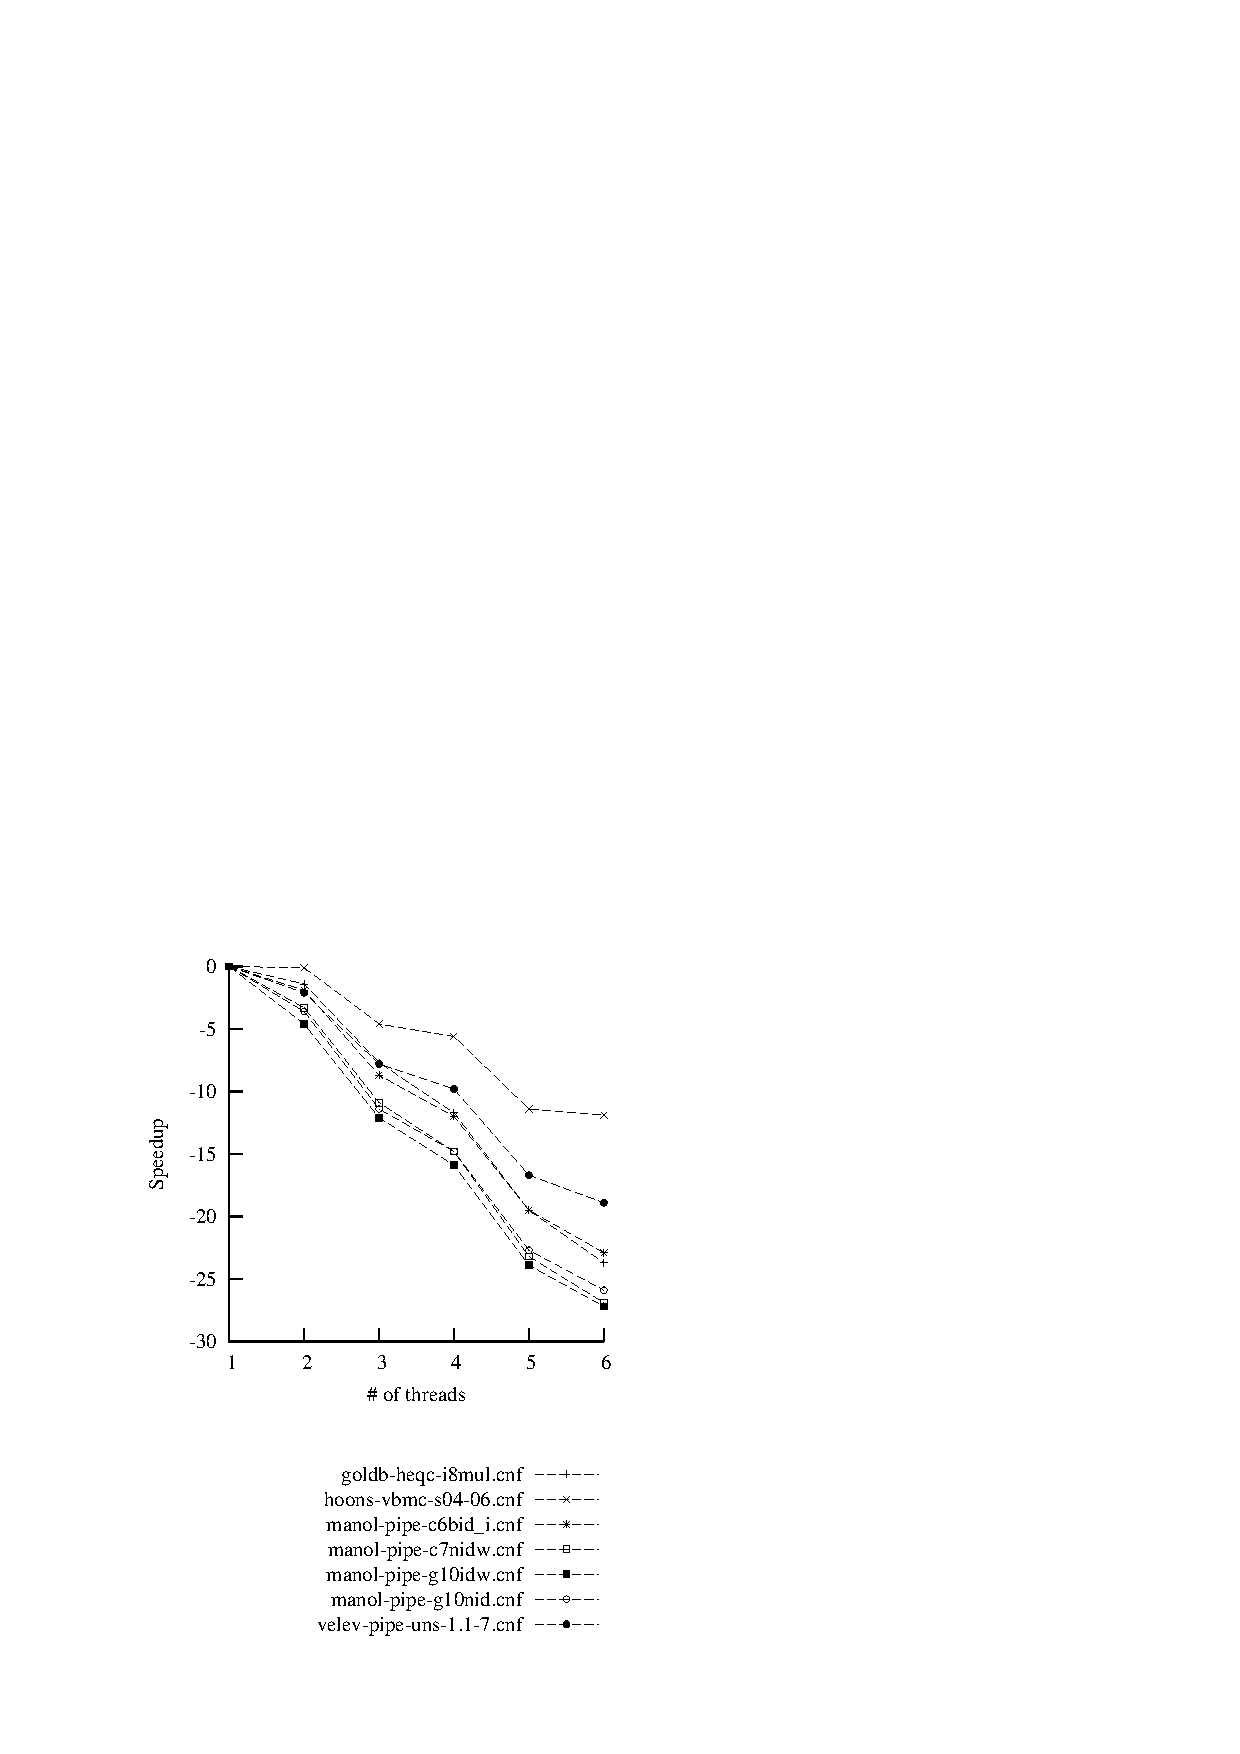
\includegraphics[width=0.7\textwidth]{plingeling_decay}
	\caption{Decay of plingeling solver performance when adding threads.}
	\label{fig:plingeling decay}
\end{figure}

Because portfolio approach SAT solvers implement different search strategies among their solving threads, it is hard to measure the real impact in performance of adding an extra thread. The new thread might implement a successful search strategy, which will make the total solving time improve drastically and hide the negative impact in the cache performance when adding a new thread. This is why we have modified \texttt{plingeling} to make the exact same search in all of its threads. In theory, we would expect the solver to finish at the same time with one thread than with $n$ threads, because all threads are performing the exact same search and thus should finish at the same time. But we know that each solver thread also keeps its own clause database, so basing our reasoning on the previous experiment, we should expect that adding threads will hinder the overall solver performance. This modified \texttt{plingeling} solver with $n$ threads should perform worse as $n$ grows, assuming that we have enough cores to run $n$ threads and that all cores belong to a same chip. Figure \ref{fig:plingeling decay} shows how the \texttt{plingeling} solver decreases its performance as we add more threads. Each line represents a different benchmark SAT problem, the X axis is the number of threads being used, and the Y axis is the speedup obtained, which is a percentage of decrease in total solving time. The decrease in performance is very noticeable and it can even reach close to 30\%. Our first hypothesis is that this decrease in performance is mostly due to cache issues.

\begin{figure}[h!]
\begin{center}
	\subfloat[Same Chip]{\label{fig:same chip}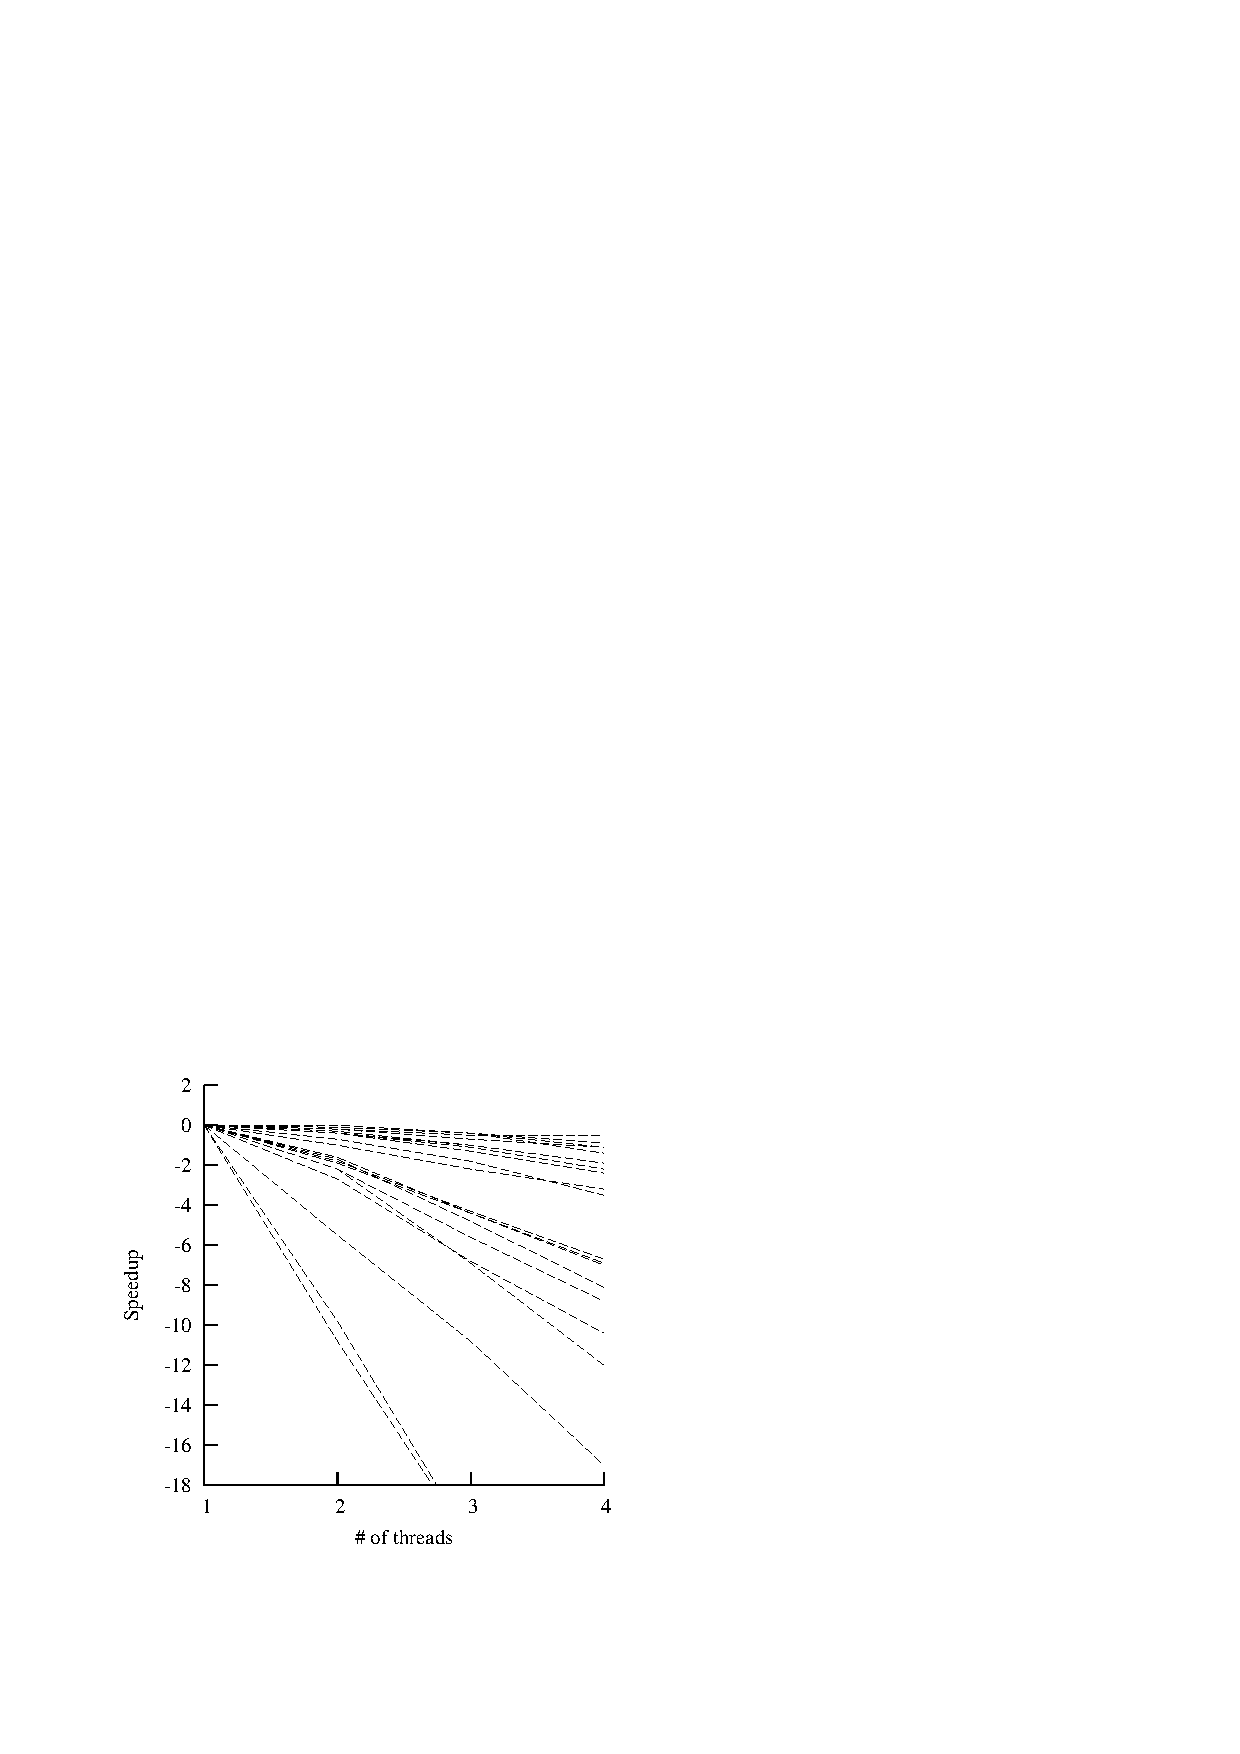
\includegraphics[bb=59 90 294 325,clip,width=0.5\textwidth]{plingeling_same_chip}}
	\subfloat[Different Chips]{\label{fig:different chip}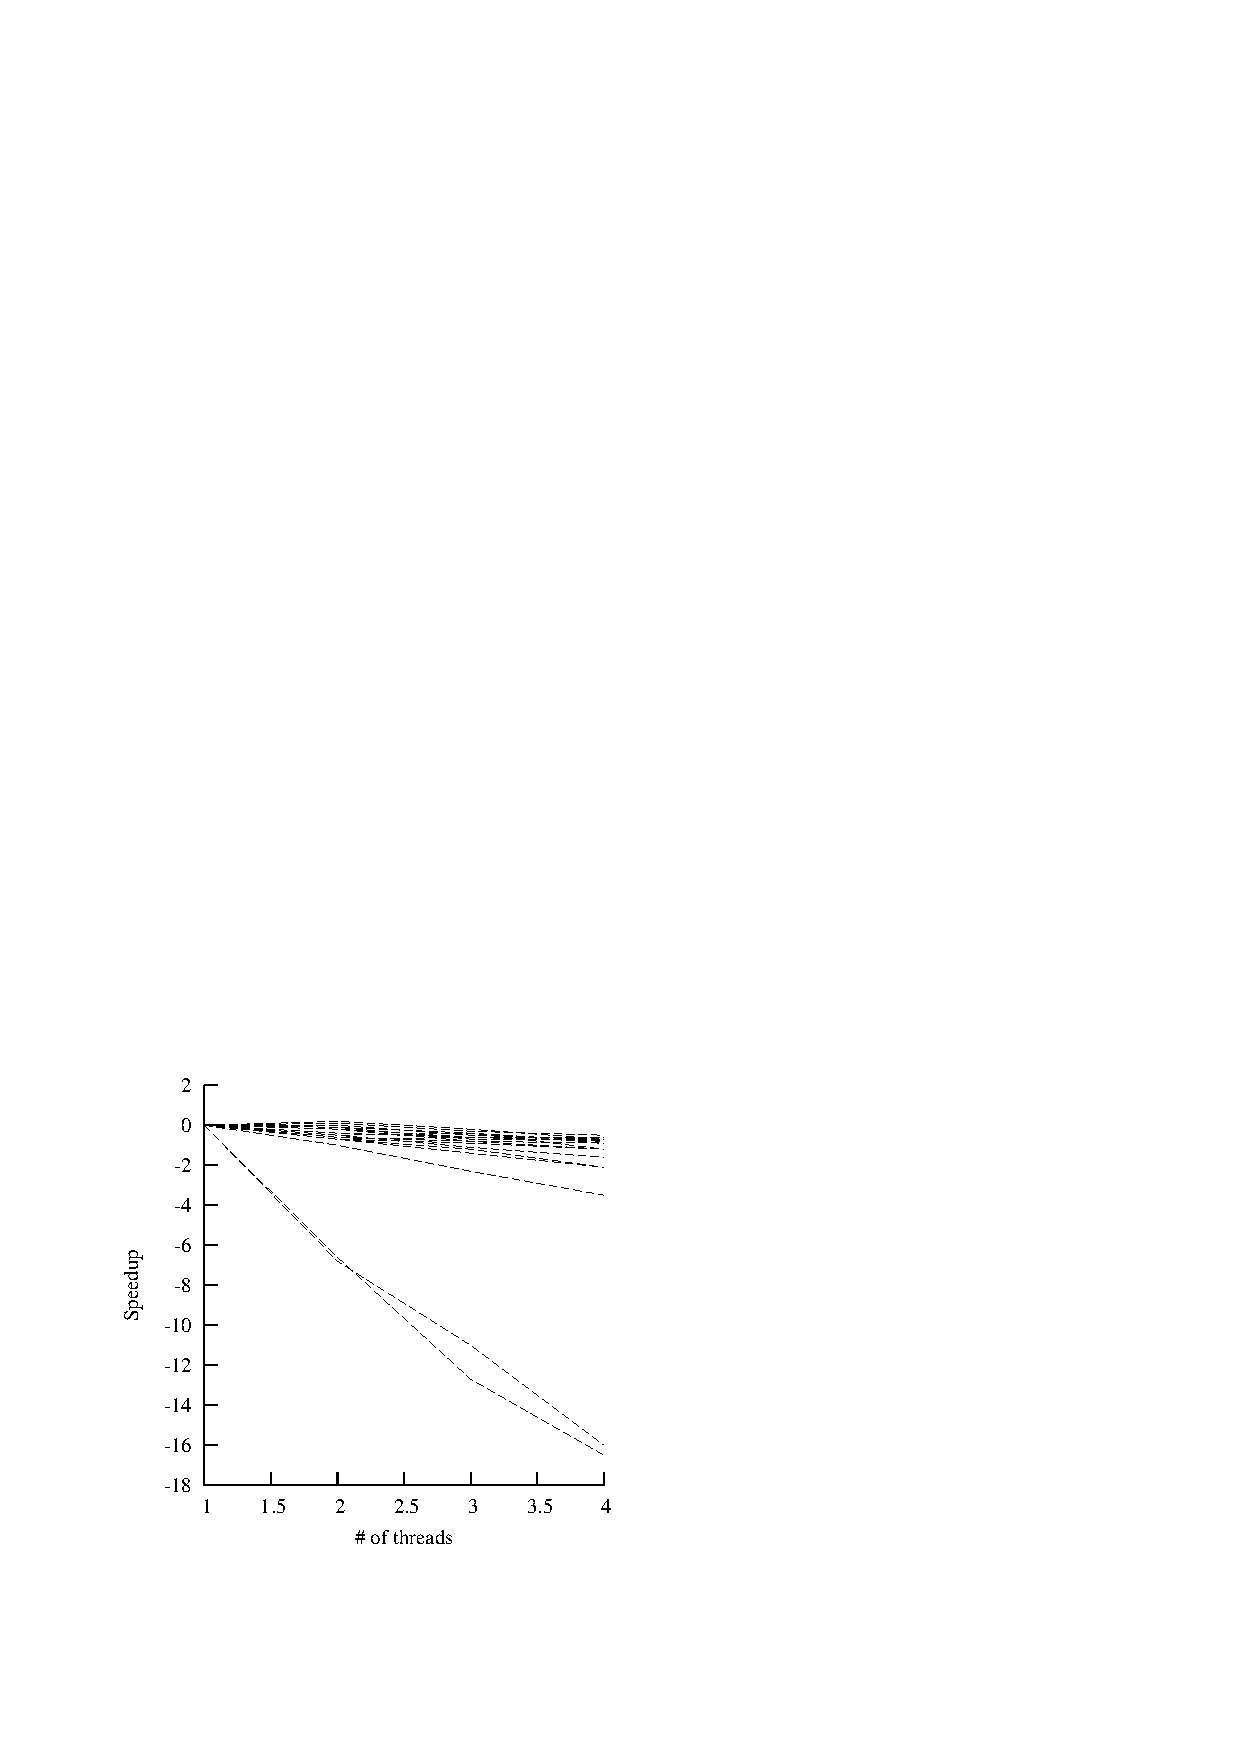
\includegraphics[bb=59 90 294 325,clip,width=0.5\textwidth]{plingeling_different_chip}}
	\caption{\texttt{plingeling} performance on different machine set ups.}
	\label{fig:plingeling chips}
\end{center}
\end{figure}

To prove that the problem in scalability lies in cache, we have also performed the experiment on a four chip machine, running each different thread in a different chip. As chips have their own last level cache, we expect the performance decrease to be minimal as we add threads, because different threads will not be sharing cache. Figure ~\subref*{fig:different chip} shows the decrease in performance as we add threads in separate chips. We can observe that the performance decrease in this case is minimal for most problems (only around 1-2\%), contrary to the situation where threads are in different cores of a same chip (where many problems exceed -4\% decrease), as shown in Figure ~\subref*{fig:same chip}. The fundamental difference between the two set ups used is that cores in the same chip share the LLC, while cores in different ships have their own LLC and only share main memory. Each solver has its own database of clauses, so the more LLC memory it has at its disposal, the better it will perform individually. The two problems for which the performance decay is noticeable in Figure \ref{fig:plingeling chips} (the two bottom lines in both graphs), are files which contain an unusual large amount of clauses, so a considerable amount of time is spent parsing the input file and generating the clause database. Because \texttt{plingeling} parses a file and then generates a new clause database for each thread, this operation takes even more time when we have multiple threads, and this is why we see that considerable performance decay on different chips for those two particular files. This particular kind of performance decay is different to the one being studied in this report, we are mostly interested in the decay related to cache behaviour in the propagation process, rather than clause database initialization. On a hard problem, which we are mostly interested in, the time spent initializing the databases should be negligible compared to the time spend solving the problem. On the contrary, on an easy problem with a large amount of initial clauses, the solver will spend a significant amount of total time initializing the thread databases. 

%Table \ref{tab:plingeling cache} shows the cache miss percentages as we add more threads to a solver that runs on a single chip. As suggested by our hypothesis, the LLC miss percentage increases dramatically as we add threads, results that explain the decrease in performance of the solver.

\section{A parallel portfolio approach SAT solver with physically shared clause database: AzuDICI}

It is now clear that as we add more data to a SAT solver clause database, we make its performance decrease because of the cache misses involved in handling a bigger volume of data. We will now perform an analysis on how well does sharing data in SAT solvers help reduce the cache misses as we add threads. To be able to do such analysis, we implemented AzuDICI: a portfolio-approach SAT solver that shares clauses physically. As we mentioned earlier, there are other solvers which implement physically shared clause databases, but they do not make a detailed analysis of the cache performance of such solvers, which will be the contribution of our experiments with AzuDICI.

\subsection{General outline}

AzuDICI\footnote{You can find the latest implementation of AzuDICI at
  \url{https://github.com/leoferres/AzuDICI}} is a standard CDCL
solver mostly based on {\tt barcelogic} and {\tt miraXT}. In particular, AzuDICI implements binary implication lists for the
propagation with binary clauses, and the two-watched literals scheme
for unit propagation with clauses of more than two
literals. For the multithreaded versions that share clauses, the two-watched literals scheme has been modified and it will be explained later in this chapter. For conflict detection and clause learning, AzuDICI implements the 1-UIP algorithm. A lemma simplification algorithm is used for new learnt clauses, it's the same used in {\tt
  PicoSAT}. For search restarts it uses Luby restarts \cite{Luby}. For database database clean up it keeps binary and ternary lemmas, and more than four-literal
lemmas that have participated in a conflict since the last
cleanup. Finally, AzuDICI also incorporates the EVSIDS heuristic for
branching literal decisions.

To allow a a comparison of clause sharing in these kind of SAT solvers, AzuDICI comes in three flavours: AzuDICI-SharedAll, AzuDICI-SharedBinaries and AzuDICI-SharedNone.

\subsection{AzuDICI-SharedNone}

\begin{figure}[h!]
	\centering
		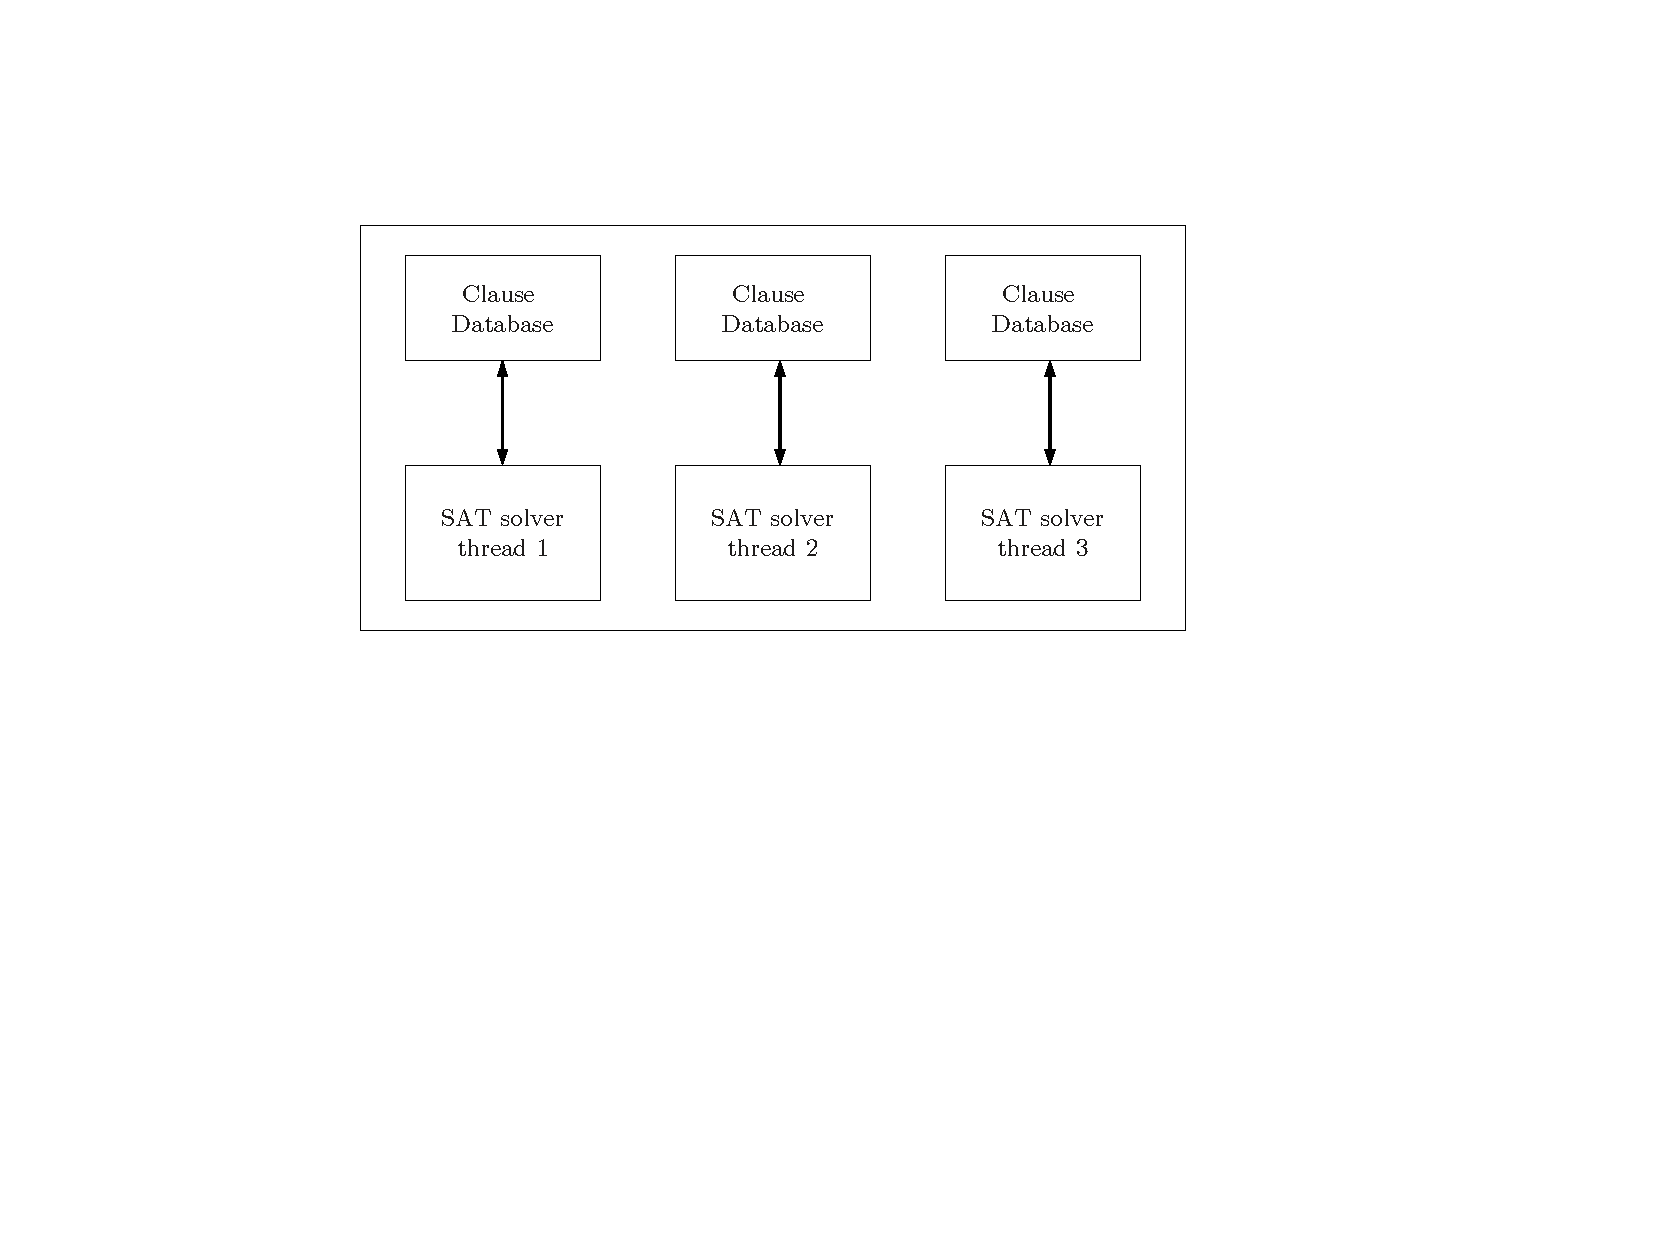
\includegraphics[width=0.7\textwidth]{sharednone}
	\caption{Three threads in an AzuDICI-SharedNone solver.}
	\label{fig:azu sharednone}
\end{figure}

This solver is a pure portfolio approach CDCL SAT solver implementation that doesn't share any kind of clause. Each thread has its own AzuDICI sequential solver and its own clause database, Figure \ref{fig:azu sharednone} is a schematization of the solver's internal structure. No locks or special data structures are required for this version, since we do not share any clauses (logically or physically), there are only completely independent solvers working on each thread. Each solver will have a different search, because they will use different random values for its heuristics.

\subsection{AzuDICI-SharedBinaries}

\begin{figure}[h!]
	\centering
		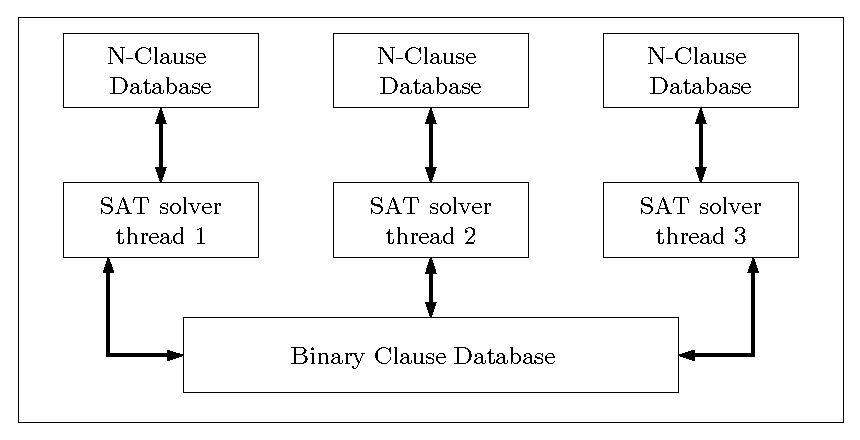
\includegraphics[width=0.7\textwidth]{sharedbinaries}
	\caption{Three threads in an AzuDICI-SharedBinaries solver.}
	\label{fig:azu sharedbinaries}
\end{figure}

This solver shares binary clauses between its threads physically. All threads have access to the same binary implication lists and they can read and add binary clauses when necessary. Figure \ref{fig:azu sharedbinaries} shows the structure of this solver. Each thread has its own n-clause database, but they all share the same source of binary clauses. The advantage of this approach over sharing everything, is that a shared implication list of binary clauses is simple to implement and does not add significant overhead to the overall performance of the solver. This is because we do not need to keep additional information for each thread and propagation works the same way as it would without sharing the binary clause database.

\begin{figure}[tp]
  \centering
  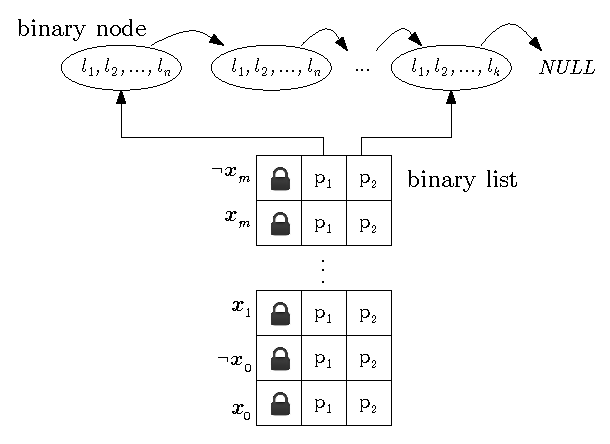
\includegraphics[scale=1.0]{implication_list}
  \caption{Binary clause database}
  \label{fig:shared bins}
\end{figure}

The implication list used in AzuDICI differs in some aspects to the one studied in the previous chapters. Figure \ref{fig:shared bins} is a schematization of our 
binary implication lists structure. We have an array of \textit{binary 
lists}, one for each literal. A binary list is basically two pointers, 
one to a first \textit{binary node} and another to the last binary node 
associated with that list. A 
binary node is an array of literals that also has a pointer to another 
binary node. The amount of literals a binary node can hold will depend 
on the size of the cache line we are working with; it will have as many 
literals as a cache line can hold. The literals implied by the literal 
associated to a binary list will be the ones in the binary node 
referenced by that binary list pointer and the subsequently referenced 
binary nodes. 

When a thread wants to add the clause $\{l_i,l_j\}$, it must look for 
the binary list associated with $\neg l_i$ and go to the last node linked 
to that binary list. If there is enough space in that node to add 
another literal, then it adds $l_j$. If the node is full, then it must 
create a new node with the $l_j$ literal, insert it at the end of the 
linked list of nodes, 
updating the binary list last node pointer. It does the same for the 
binary list of $\neg l_j$.

To ensure consistency of 
data when multiple threads are inserting, each binary list has a lock. 
If a thread is inserting a new implicated literal, it first locks the 
binary list where it is inserting and then proceeds to insert. If, by 
chance, another thread wants to insert in the same binary list, it must 
wait until the lock is freed. Since adding binary clauses is not a 
frequent event, and even less frequent the event that it would happen 
in the same binary list, the contention that these locks generate is 
unnoticeable in our experiments.

Another feature that sharing binary clauses brings in is that it adds another random factor to the search. Since threads are not synchronized with each other, they can add new binary clauses to the database at any given time, action that would affect the search of other threads (because they now have an extra clause to propagate with). If we were to try and replicate the exact same search as used in a particular instance of an AzuDICI-SharedNone solver, we would fail, because sharing binary clauses among threads also affects the search path of each individual thread.

\subsection{AzuDICI-SharedAll}

\begin{figure}[h!]
	\centering
		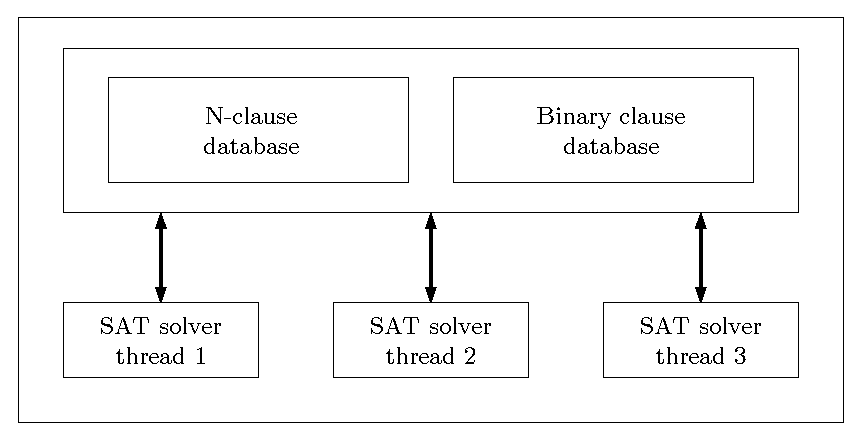
\includegraphics[width=0.7\textwidth]{sharedall}
	\caption{Three threads in an AzuDICI-SharedAll solver.}
	\label{fig:azu sharedall}
\end{figure}

This version physically shares all clauses between threads, as shown in Figure \ref{fig:azu sharedall}. The complexity, compared to the previous versions, of implementing such solver lies in the propagation on n-clauses. In a sequential solver, the two-watched-literal
scheme is usually implemented in a way that makes changes to the clause in order to identify
the literals being watched at one given instant(for example, place
both literals first in the clause). Since many threads will be
accessing the same clauses. These changes to the clause are not
feasible when sharing n-ary clauses, because multiple threads can modify the position of literals. Instead, we have used a similar 
approach as used in
{\tt miraXT}, where each thread keeps track of the literals being
watched in each clause. Figure \ref{fig:azu design} is a
schematization of how each thread worker relates with the n-ary
clause database. Each SAT solver thread has a vector of pointers
to \textit{thread clauses} called \textit{watches}, and each literal present
in the SAT problem has a position associated in this watches vector.
A thread clause is just a reference to an actual n-clause, which keeps extra information the threads needs. It has two watched literals (WL0 and WL1), two
pointers to other thread clauses (NW0 and NW1) and a pointer to
the actual n-ary clause in the n-ary shared clause database. WL0 and WL1 keep
track of the literals being watched by the thread for a given n-ary
clause. NW0 and NW1 point to the next thread clauses that are also 
watching WL0 and WL1. The n-clause also has a set of flags, one for 
each worker thread for them to identify which ones are using that clause 
for propagation.

\begin{figure}[tp]
  \centering
  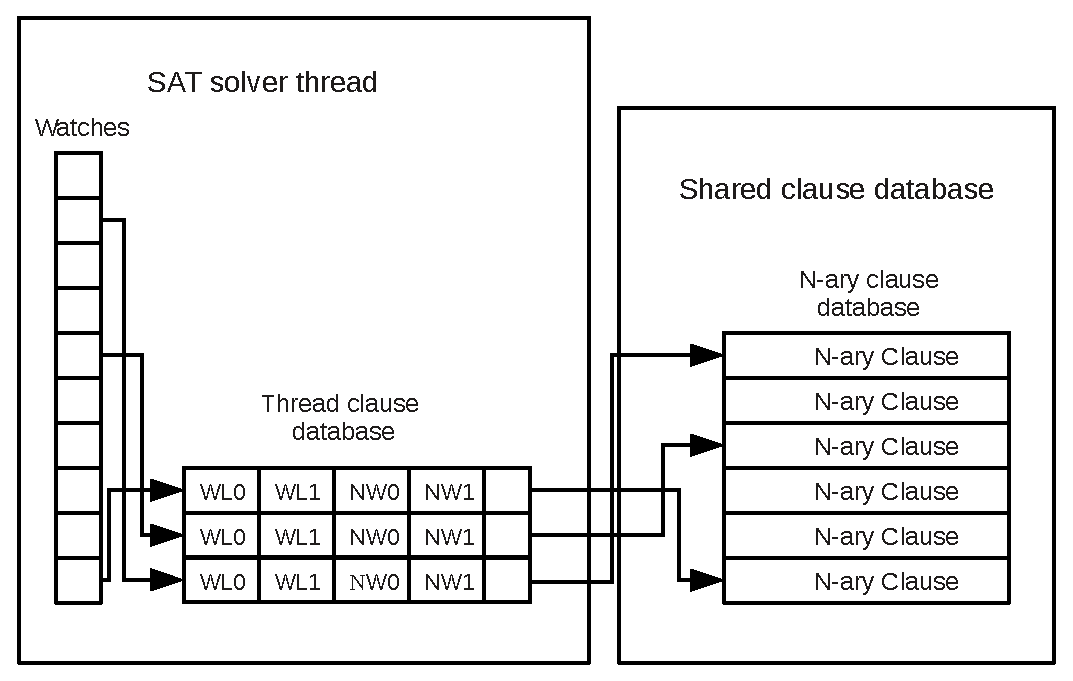
\includegraphics[scale=0.6]{AzuDICI_design}
  \caption{The thread clause database and n-ary clause database}
  \label{fig:azu design}
\end{figure}

To insert a new n-ary clause, we first make sure that the clause 
does not exist in the database. If it 
does not exist, we create the n-clause, set the current thread 
flag to true and add it to the database. 
On the other hand, if it does exist, we just toggle the 
corresponding thread flag of the n-clause to true. The inserting 
procedure is locked so that two different threads can not insert
at the same time. In our experiments we have not noticed any 
considerable overhead caused by this lock.


\section{Experimental results} 

Since we are interested in studying the cache performance of parallel SAT solvers, we will use a benchmark set of SAT problems (all used in previous SAT competitions) which we know that any of the AzuDICI versions can not solve in a defined time frame limit. This time limit was set to five minutes for our experiments. We would not want to use problems that can be solved in our time limit frame mostly because the results would be strongly influenced by the different search paths each version takes. A version that solves a problem faster due to finding a better search path will probably have a better cache performance, not because it is more cache-friendly, but because it finished before the amount of data to handle was too big.

The experiment will consist on measuring the cache performance of a solver before the timeout of five minutes. For each problem, we will ran instance of the solver with one to up to $n$ threads, and see how well cache behaves for that particular problem.

\subsection{AzuDICI-SharedNone results}

\begin{figure}[h!]
	\centering
		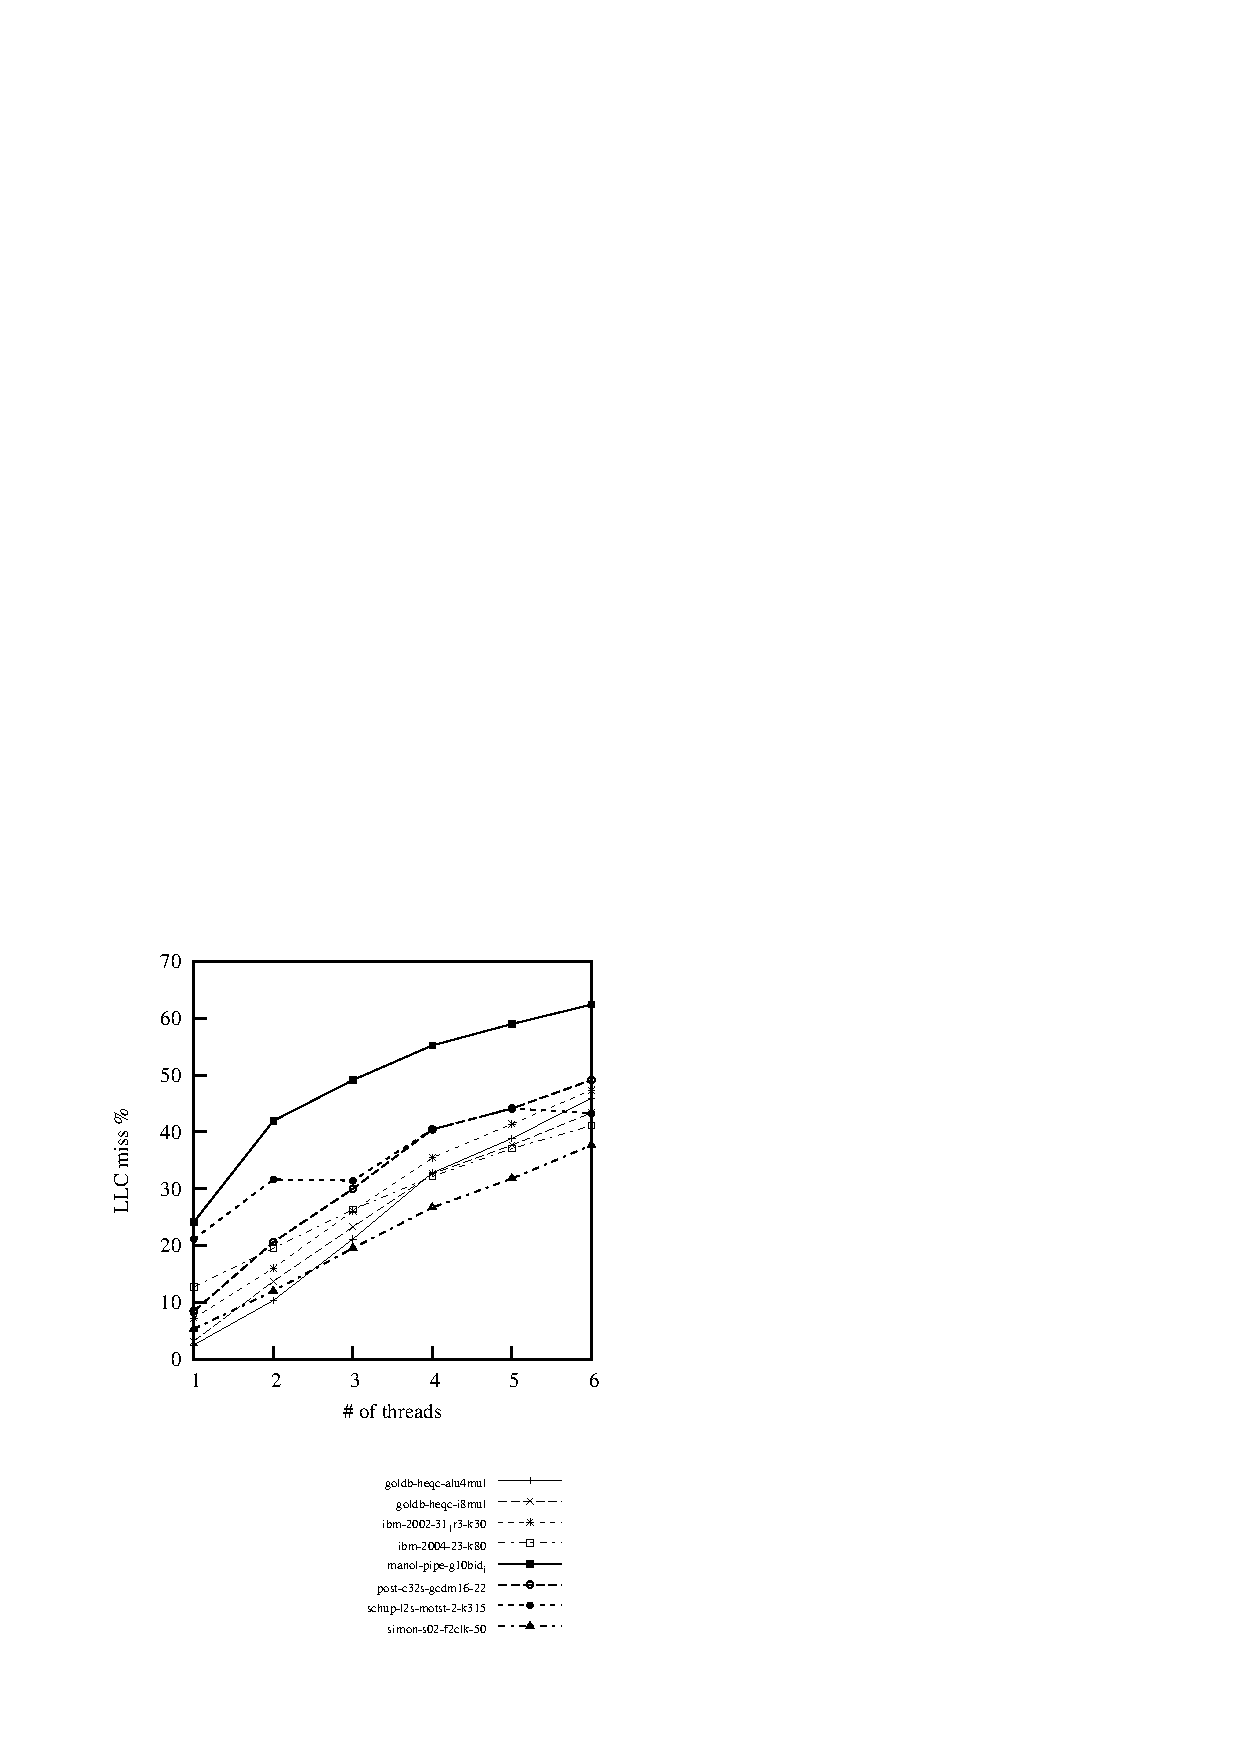
\includegraphics[width=0.7\textwidth]{shared-none}
	\caption{SharedNone experiment}
	\label{fig:shared-none}
\end{figure}

In this experiment we ran the SharedNone version with our set of benchmark problems. Figure \ref{fig:shared-none} shows the results for this experiment. As we expected, the cache performance decreases as we add more threads, the LLC miss percentage jumps from around 5-10\%, for one thread, to about 35-50\% when running on six threads. The overall scaling for all problems is poor and the continuous increment in LLC misses suggests that the propagation of clauses is much more slower when working with multiple threads. We can infer from this graph that if we continue adding threads (assuming we had enough cores), the cache performance would be so low that it would not be beneficial to add any more threads, as the propagation of clauses would be too slow to add any improvement. Unfortunately, finding this point, where adding more threads becomes counter productive, should be very difficult, because each problem may show a very different behaviour and each new thread might also behave very differently, yielding different optimal number of threads. We could perform a statistical study over a very large sample of benchmark problems to find that number of optimal threads for a typical SAT problem, but we will leave such experiment for future work. For now, we are only interested in knowing that when we don't share clauses physically, the scaling of cache performance is poor.

\subsection{AzuDICI-SharedBinaries results}

\begin{figure}[h!]
	\centering
		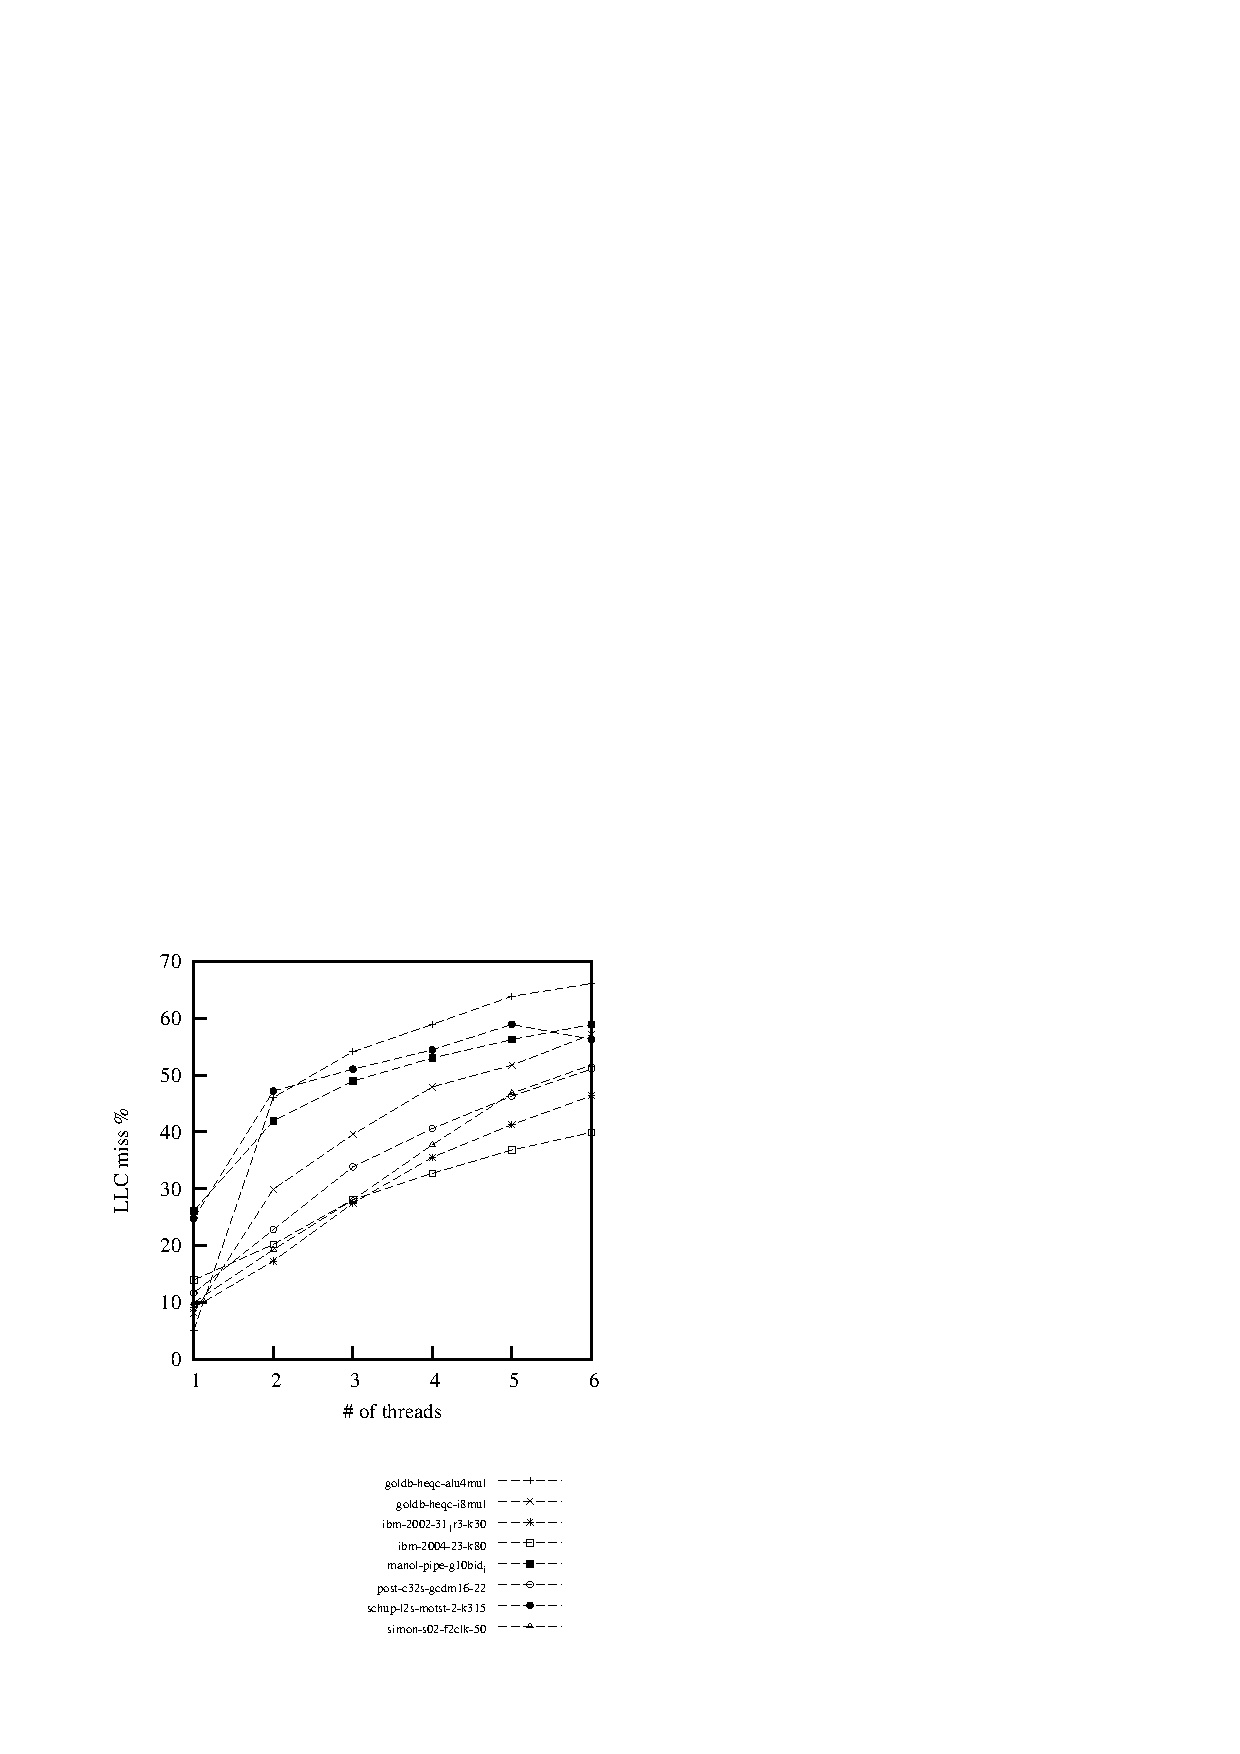
\includegraphics[width=0.7\textwidth]{shared-binaries}
	\caption{SharedBinaries experiment}
	\label{fig:shared-binaries}
\end{figure}

Figure \ref{fig:shared-binaries} shows the results in this experiment and we can observe they are similar to the SharedNone results. This can be expected as we are only sharing a small amount of clauses physically and not making any significant change to the solver. The propagation scheme is still the same for both versions. Only a small improvement, not more than a mere 2\% in most cases, in cache performance can be noticed throughout the different benchmark files. This experiment is an intermediate example of clause sharing as we only share binary ones. Once again, we see that the overall scaling as we add threads is poor and that there should be a point when adding more threads is counter productive, just as in the previous version.

\subsection{AzuDICI-SharedAll results}

\begin{figure}[h!]
	\centering
		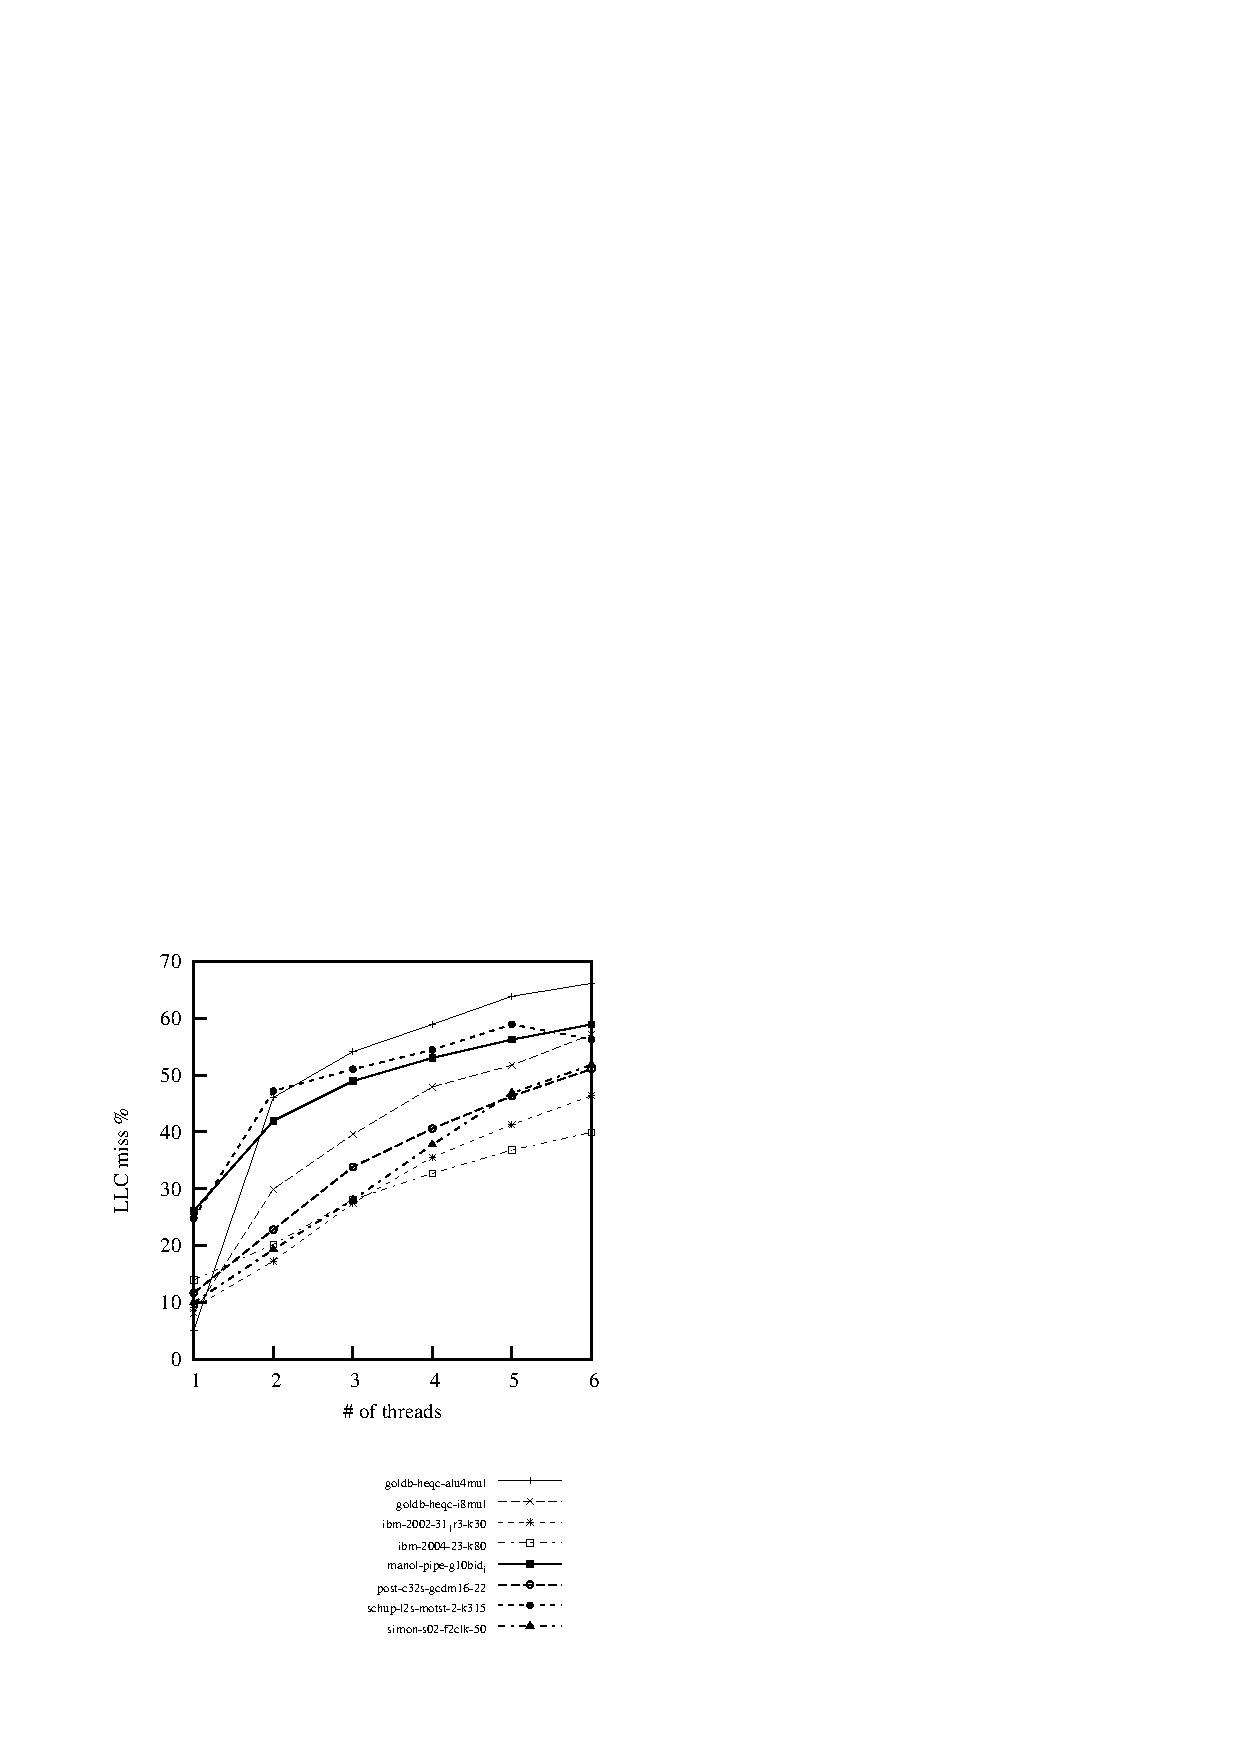
\includegraphics[width=0.7\textwidth]{shared-all}
	\caption{SharedAll experiment}
	\label{fig:shared-all}
\end{figure}

The results for this last version are shown in Figure \ref{fig:shared-all}. We expected the scaling of this solver to be much better than the previous versions, because sharing all clauses between threads lowers down the amount of total data to handle and should keep the cache misses under control, but our results show otherwise. Not only did this SharedAll version not achieve the desired improved scalability, it also makes the amount of cache misses higher for all number of threads. Our explanation for this behaviour is that this solver keeps more information and has to perform additional tasks when propagating. Unlike the SharedNone version, this one needs extra structures for each thread, which keep track of the watched literals of each thread and which clauses are being used. We suspect that this additional data, plus the fact that we have to be constantly checking it during propagation, makes the cache perform even worse and totally opaque the benefits of sharing information. Also, as we described in an earlier section of this work, the amount of information to handle might be so big that it won't even matter if we share it, the size of it can still be too big to have a better chance of finding data in the LLC.

\begin{figure}[h!]
	\centering
		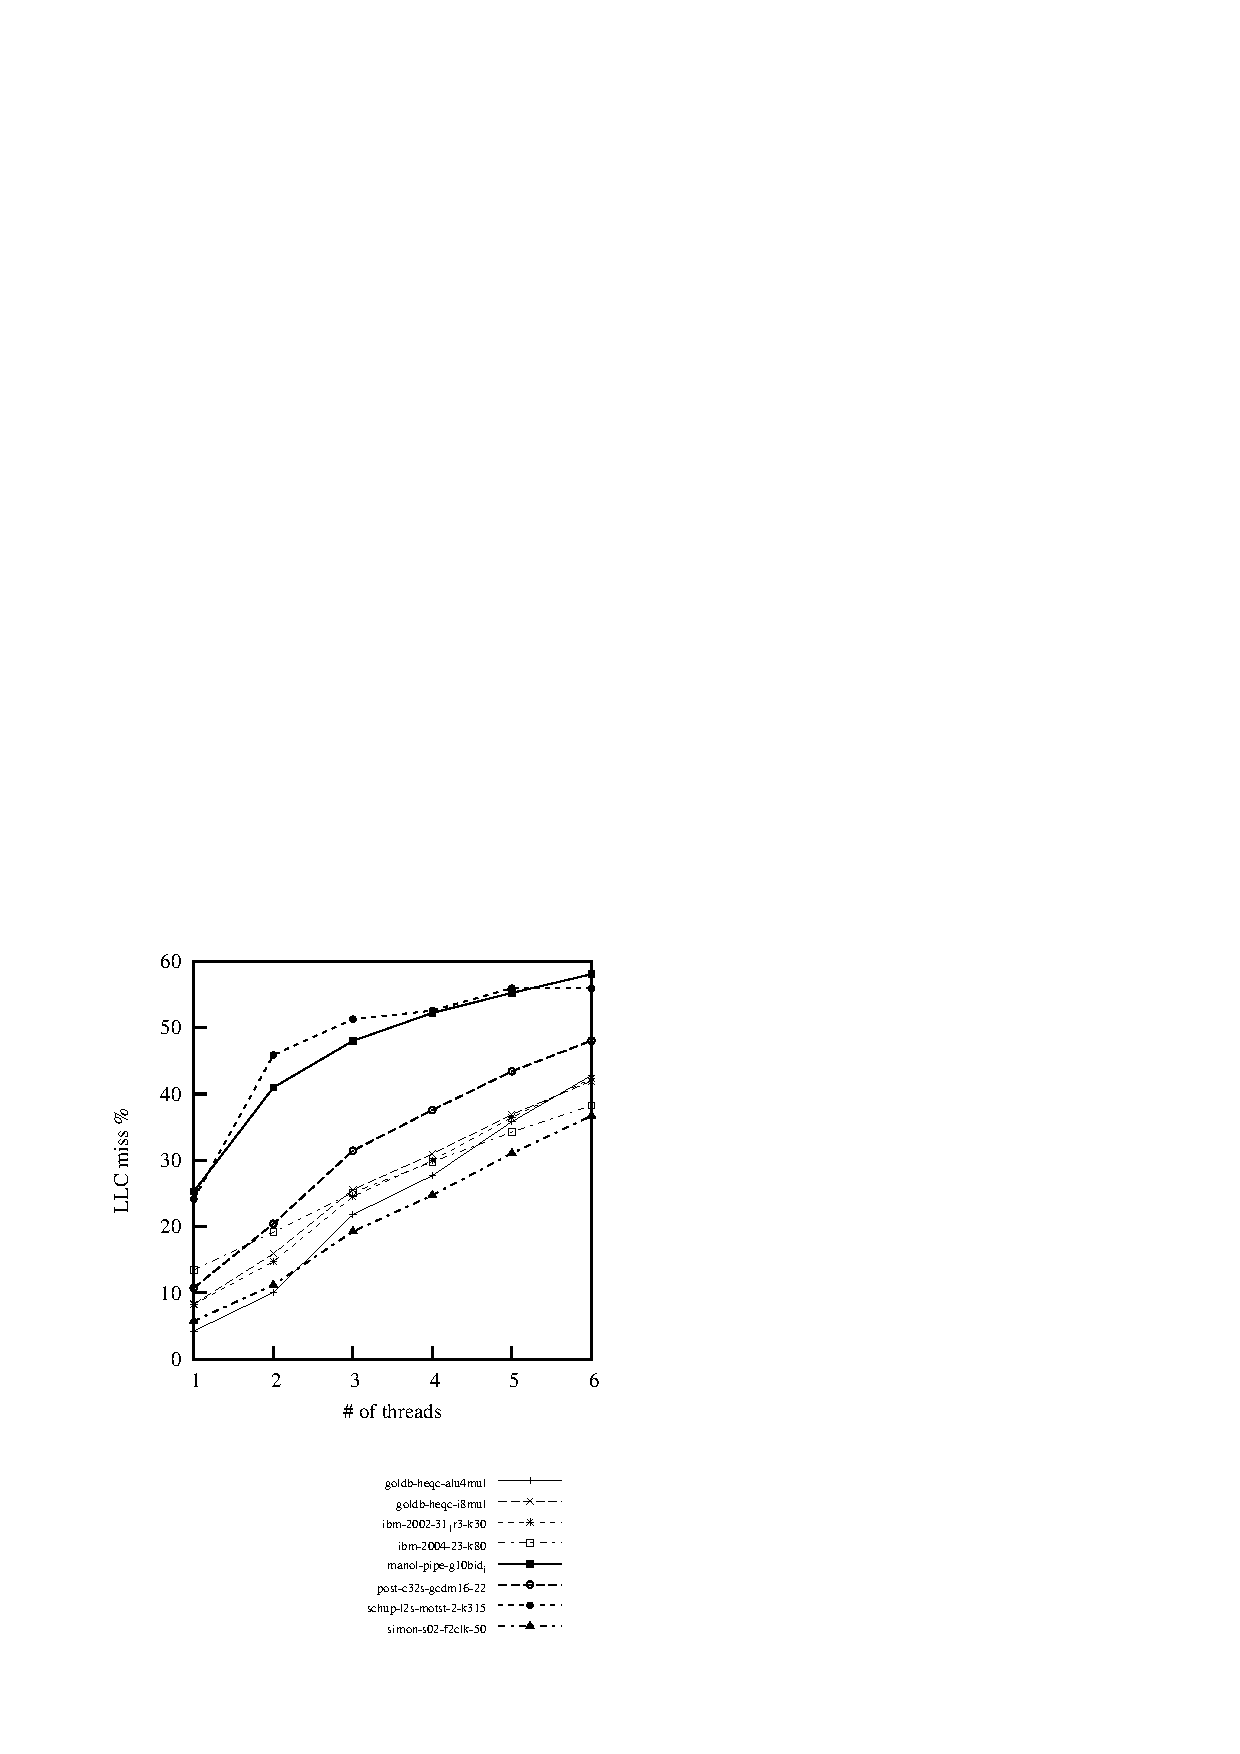
\includegraphics[width=0.7\textwidth]{shared-all-start}
	\caption{SharedAllLimited experiment}
	\label{fig:shared-all-start}
\end{figure}

We also did an extra experiment with a new solver version, which only shares the initial clauses read from the input file, and then keeps separate clause databases for the new learnt clauses. We called this new version SharedAllLimited and Figure \ref{fig:shared-all-start} shows the results of such experiment. We can observe that the results improve compared to SharedAll and we end up getting lower LLC miss percentage, but similar numbers to the SharedNone and SharedBinaries versions.

\subsection{Summing it all up}

\begin{figure}[h!]
	\centering
		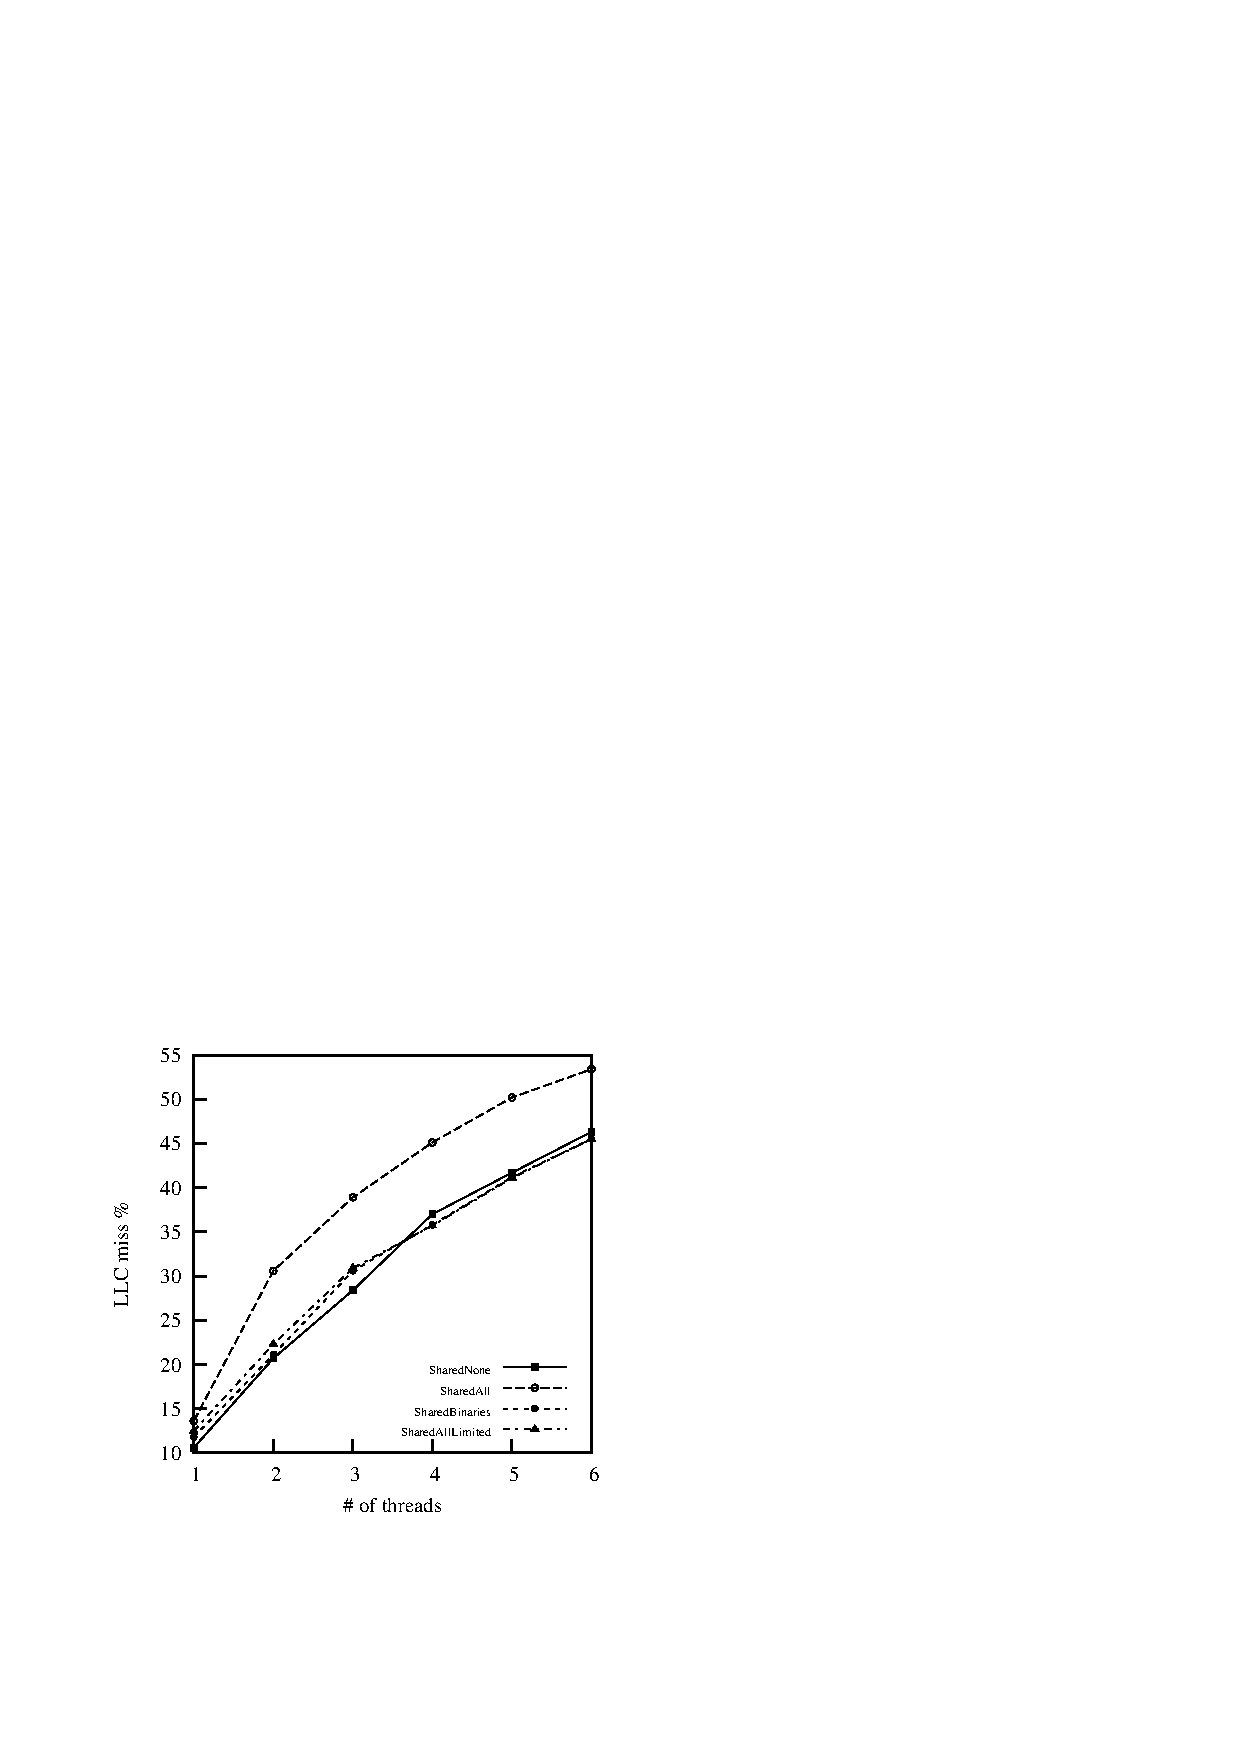
\includegraphics[width=0.7\textwidth]{average}
	\caption{Average graph}
	\label{fig:average}
\end{figure}

To get a clearer picture of our results, we have plotted the average LLC miss percentages of all problems for all versions. Figure \ref{fig:average} compares all versions averages in a single graph. We can clearly see that SharedAllLimited and SharedBinaries perform very similar and slightly better than SharedNone. This is because sharing some information, as little as it might be, does help with LLC miss percentages and does not modify the propagation scheme in any way. On the other hand, SharedAll has the worst performance, because, as we mentioned earlier, the gains of sharing clauses physically do not surpass the harms of modifying the propagation scheme and keep additional information for it.


%%%%%%%%%%%%%%%%%%%%%%%%%%%%%%%%%%%%%%%%%%%%%%%%%%%%%%%%%%%%%%%%%%%%%%%%%%%%%%%%
% Step 13: Add a conclusions chapter
%
% 
%%%%%%%%%%%%%%%%%%%%%%%%%%%%%%%%%%%%%%%%%%%%%%%%%%%%%%%%%%%%%%%%%%%%%%%%%%%%%%%%
\chapter{Conclusions}\label{chap:conclusion}

Throughout this work we have shown that algorithm design might not always be oblivious to modern computer architecture. Memory hierarchy plays an important role in the performance of both single and multi threaded applications. From our small experiments that deal with common cache problems we can conclude that we must know how modern memory architecture works to get the best performance out of our programs. This is no different in the SAT solving world, where it is already known that cache plays an essential role in the efficiency of state-of-the-art solvers. Although cache performance has been widely studied for sequential SAT solvers (mainly studies about the two-watched-literal scheme \cite{chaff}), it is yet not clear how it affects the design of parallel SAT solvers, which was the main focus of this work. We were able to prove that it is not possible to just keep adding threads to state-of-the-art parallel SAT solvers and expect to keep performing better. As we add more threads there is a considerable performance degradation of all threads, degradation that might get so high as to prove fruitless to keep adding threads.

It is also clear by now that sharing information between threads in a parallel program does help with cache performance, because of the higher chance to find data in the cache, but it is also equally important that the drawbacks of the modifications, introduced to share information, do not overwhelm the benefits. For instance, sharing information between threads will usually lead to the implementation of some type of lock, specially if the information is being modified, and locks can have a noticeable negative impact in overall performance. In our work this was not the case, but when sharing all clauses we stumbled upon the problem of having to modify the usual scheme of some of the processes involved in SAT solving. This is the reason why making multi-threaded applications is so difficult when the application is complex. There is no general rule of thumb or recipe that will work for all domains, each program has its own complexities and specific constrains that will require detailed study and experimentation in order to achieve a better parallel version. 

In the domain of parallel SAT solving, it is clear that sharing clauses among threads is a good idea and improves the search across all threads, but it is not clear which is the best way to do so. Some solvers, as we mentioned, share them through message passing and others would rather share them physically, but no real analysis of the performance of both approaches has been done. In this work we have used the approach used by \texttt{MiraXT} to share clauses physically, but our experiments and cache studies show that this is not a good idea. It is much more simple, straight forward and better to just let each thread manage its own separate clause database and avoid all the difficulties of physical sharing, which at the end only show to harm the overall cache performance of the solver. The only exception would be to physically share the unary and binary clauses, because these kind of clauses can easily be shared with no complications and significant overhead, while improving cache performance by a small margin. 

For future work we would like to perform a statistical analysis with state-of-the-art solvers, to measure the optimal number of threads that these solvers should run in one chip, so that degradation in cache performance will not overshadow the benefits of having an extra thread. We would also like to implement versions of AzuDICI which share data through message passing, not physically, and compare them to the versions from this work. Another idea we would like to explore is just keeping a fixed amount of running threads, and switch between different solvers among these threads. As we mentioned before, the problem of performance in parallel solvers becomes evident when the amount of data of all threads becomes too big for the LLC performance to be efficient. So to solve this issue we could just keep a low amount of threads and arbitrarily assign running time to each solver among these threads. For example, if we wanted to run 10 worker threads in a 10 core machine, we could infer that 10 threads will generate too much data for cache to be efficient, so we could only run 6 threads with just 5 instances of the solver for a certain period of time, then switch some threads to run the other 5 instances, and keep switching between them. By doing this we would always keep a good cache performance because we would never have more than 6 clause databases being used at the same time. The drawback would be that the switching of the different solver instances would probably cost some time (because we will need to load different clause databases and solving models each time we switch), but we would need to run experiments to come to a conclusion on whether this is a good idea or not. 

%%%%%%%%%%%%%%%%%%%%%%%%%%%%%%%%%%%%%%%%%%%%%%%%%%%%%%%%%%%%%%%%%%%%%%%%%%%%%%%%
% Step 14: Work out the bibliography
%
% 
%%%%%%%%%%%%%%%%%%%%%%%%%%%%%%%%%%%%%%%%%%%%%%%%%%%%%%%%%%%%%%%%%%%%%%%%%%%%%%%%
% Tips: 
%
% For named.bst, if I add a~\cite*{} it will add all the references I
% have in the bibliography file (whether they are referenced in the
% document or not)
%%%%%%%%%%%%%%%%%%%%%%%%%%%%%%%%%%%%%%%%%%%%%%%%%%%%%%%%%%%%%%%%%%%%%%%%%%%%%%%%
\bibliographystyle{plain}
\bibliography{biblio}

\end{document}
